% Chapter Template

\chapter{Implementing the PO-TITE-CRM trial design into ADePT-DDR} % Main chapter title

\label{Adept} % For referencing this chapter elsewhere, use \ref{Adept}

%----------------------------------------------------------------------------------------
%	SECTION 1
%----------------------------------------------------------------------------------------

\section{Introduction}
\label{adept:Introduction}

Worldwide there are approximately 600,000 new cases of Head and Neck Squamous Cell Carcinoma (HNSCC) each year \cite{stranskyMutationalLandscapeHead2011}. Of which, 12,000 occur in the UK with the most common forms of treatment being surgery, radiotherapy and/or chemotherapy \cite{cancerreaserchukHeadNeckCancers2017}. Radiotherapy is essential for the treatment of cancer. It has been estimated that more than 40\% of patients will receive radiotherapy at some point in their treatment \cite{roundRadiotherapyDemandActivity2013}. However, despite recent advancements in radiation techniques and the use of concomitant chemoradiotherapy, patients with solid tumours such as head and neck cancer have suboptimal cure rates \cite{cancerreaserchukHeadNeckCancers2017,cognettiHeadNeckCancer2008}. For those with advanced HNSCC primary radiotherapy with concurrent chemotherapy is often offered but, it has not been shown to improve survival in patients aged over 70 compared to radiotherapy alone \cite{pignonChemotherapyAddedLocoregional2000}. Therefore, any strategy to improve the efficacy of radiotherapy without increasing toxicity would have a significant impact on patient outcomes. 

DNA damage repair (DDR) inhibition is a potential technique which could be utilised as it potentiates the therapeutic effects of ionising radiation in cancer cells \cite{oconnorTargetingDNADamage2015}. Combining radiotherapy with DDR inhibition could improve clinical outcomes for these patients \cite{chalmersScienceFocusCombining2016}.  

The ADePT-DDR trial \footnote{Accelerating the Development and implementation of Personalised Treatments of DNA Damage Response agents and radiotherapy +/- immunotherapy for head and neck squamous cell cancer } is a platform trial which aims to evaluate the safety and efficacy of different DDR agents, or different immunotherapy agents and/or DDR and immunotherapy combinations, together with radiotherapy in patients with HNSCC. The initial component of this trial is a single-arm dose-finding trial investigating the ataxia telangiectasis and Rad3-related (ATR) inhibitor AZD6738 in combination with radiotherapy. ATR inhibitors not only stop DNA repair but impair the mechanism that allows for repairs to take place. Preclinical models have shown this double blocking to be effective in killing cancer cells \cite{meiAtaxiaTelangiectasiaRad3related2019}. 

In Chapter \ref{Intro} we discussed model and algorithm-based dose-finding trial designs. Due to the historical use of rule-based designs \cite{rogatkoTranslationInnovativeDesigns2007, chiuzanDosefindingDesignsTrials2017}, the majority of the terminology used to describe them, and the ambiguity they raise, have been inherited by modern designs such as the CRM. The MTD in the context of a CRM is not the 'maximum' dose patients could tolerate but rather a dose in which there would be an acceptable target probability of a DLT occurring. For example, if the target is set at 25\% the MTD would be the dose at which there is a 25\% probability of experiencing a DLT. Rather than using the term MTD, the dose to be found will be referred to as the target dose (TD\%\%, where the \%'s are replaced by the target probability), i.e. TD25 would be the dose expected to be toxic in 25\% of patients.

The investigation of multiple-agent treatments, where the monotonicity assumption may not hold, is increasing in early phase trials. Finding the TD in combinations of treatments, compared to single-agents,  presents methodological challenges. Each drug individually may obey the monotonicity assumption; we can refer to this as the doses being fully ordered. However, when multiple treatments are combined, the ordering of doses in terms of toxicity may not be fully apparent or may only be partially defined. An order may be identified for a subset of the doses which would result in a partial order. Without a full ordering it is uncertain which dose should be chosen in decisions of escalation and de-escalation and ultimately as the TD. This issue is not exclusively reserved for trials with multiple-agents. The monotonicity assumption may not hold for certain drugs in single-agent studies leading to partial orders of dose toxicity. For example, when dose and frequency of administration vary between dose levels. It requires that probability of toxicity always increases - staying the same is not enough. At high enough doses, this assumption is almost surely violated for all interventions when the event probability reaches its maximum. Thus, even when total ordering is possible, the monotonicity assumption could be violated \cite{brockMoreBetterAnalysis2021}. Issues of partial ordering can occur in scenarios where multiple parameters of the treatment schedule are altered for each dose level. For example, either dose or treatment duration could be increased and even if patients receive an equal dose it would remain unclear as to if prolonged exposure to a lower dose is more toxic than short exposure to a higher dose, which implies a partial ordering of toxicity probabilities. 

Further methodological challenges revolve around the issue of late-onset toxicities. Typically, early phase trials implement a short window to observe DLTs. This works well in situations where toxicities are likely to occur rapidly after treatment. However, this is not optimal for treatments that could cause late-onset toxicities such as radiotherapy. The aim with ADePT-DDR would be to incorporate a larger observation window to account for potential late-onset toxicities whilst also minimising the trial duration. 

Cheung and Chappel \cite{cheungSequentialDesignsPhase2000} introduced an extension to the CRM to deal with the issues of treatments that may cause late-onset toxicity. This design referred to as the time-to-event CRM (TITE-CRM), uses a weighted dose-response model to incorporate the time it takes for a DLT to occur in a patient. There have also been published trial designs to deal with the issues that arise from investigating combinations of treatments. Thall et al. \cite{thallDoseFindingTwoAgents2003} proposed an adaptive two-stage Bayesian design which utilises a parametric model of toxicity as a function of two doses. Yin and Yuan \cite{yinBayesianDoseFinding2009} present a Bayesian design that uses a copula regression model to evaluate the joint toxicity probabilities of combined drugs. The continual reassessment method for partial orders (PO-CRM) developed by Wages et al. \cite{wagesContinualReassessmentMethod2011} extends the CRM design by relaxing the assumption of monotonicity and by modelling different potential orders. Figure \ref{fig_adept:example_dose_levels} shows a simple example of partial ordering where the order of two out of the four dose levels are unknown. 

\begin{figure}[h!]
	\centering
	\caption{Example dose levels to illustrate partial ordering.}
	\label{fig_adept:example_dose_levels}
	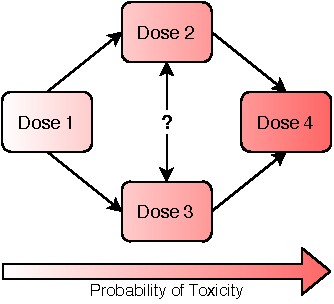
\includegraphics[width=0.75\textwidth]{Adept-DoseExample}
\end{figure}

Wages et al. \cite{wagesUsingTimetoeventContinual2013}, \cite{wagesContinualReassessmentMethod2011} further developed their work on the PO-CRM to deal with late-onset toxicities by implementing a TITE component. This trial design, referred to as the time-to-event continual reassessment method in the presence of partial orders (PO-TITE-CRM) by the authors, was chosen to be used in ADePT-DDR. A search of PubMed, conducted on the 25th of July 2020, found six articles that had cited the PO-TITE-CRM design by Wages et al. \cite{wagesUsingTimetoeventContinual2013}. Of these six articles non actually implement the design into a trial. The following paragraphs provide more details. 

Five of these papers were methodological in nature, two of which only include the PO-TITE-CRM design in a brief introduction to current methodology before going on to present new Bayesian trial designs \cite{liuBAYESIANDATAAUGMENTATION2013, wheelerBayesianModelfreeApproach2019}. The other three papers were authored by Wages. The first of which details practical considerations and specifications for the PO-CRM design, the TITE variant is only cited as the source of an example which is being used \cite{wagesSpecificationsContinualReassessment2013}. One paper presents an R package 'pocrm' \cite{wagesPocrmRpackagePhase2013, wagesPocrmDoseFinding2019}. The package is only capable of analysing the PO-CRM design. The TITE variant is only referenced here as it illustrates the issue of partial ordering. The last methodological paper by Wages et al. \cite{wagesPracticalDesignsPhase2016} presents three different methods for phase \RN{1} studies of drug combinations one of which is the PO-CRM however, PO-TITE-CRM is only mentioned as an extension to this design. A key message in this paper is the fact that novel methodologies are constantly emerging but are rarely implemented in practice. 

The last paper is a protocol paper for a phase \RN{1}/\RN{2} study, OLA-TMZ-RTE-01 \cite{lesueurPhaseIIaStudy2019}. The phase \RN{1} component of the study aims to determine the recommended phase \RN{2} dose (RP2D) of olaparib combined with a standard schedule of radiotherapy and temozolomide (TMZ) as first line treatment for patients with unresectable glioblastoma (GBM). The treatment schedule is divided into a radiotherapy and maintenance period. They propose to conduct two sequential dose-escalations of seven different  olaparib dose-levels. Patients in the first escalation will be allocated to a dose level of olaparib for 10 weeks including radiotherapy for six weeks with TMZ given each day during radiotherapy and then for six cycles four weeks post radiotherapy during the maintenance period. They state the MTD1 will be determined using a TITE-CRM. Patients in the second escalation olaparib at the MTD1 during the radiotherapy period along with the same schedule of radiotherapy and TMZ. Those patients will then be allocated to one of the seven dose levels of olaparib during the maintenance period. Again, it is stated that the MTD2 will be determined using TITE-CRM modelling. The RP2D is the MTD1 and MTD2 during the radiotherapy and maintenance period respectively. Even though a combination of treatments is being investigated only olaparib is being escalated and doses for other treatments are fixed for all patients. Furthermore, the dose-levels for olaparib increase consistently in either amount or duration meaning there are no issues of partial ordering which would warrant the use of PO-TITE-CRM. The authors reference the TITE-CRM methodology with two papers. One of them being the paper detailing the PO-TITE-CRM design and the other being a paper by Huang and Kuan \cite{huangTimetoeventContinualReassessment2014} which proposes an adaptive weight function that incorporates cyclical data of treatment into the TITE-CRM. It is unclear as to why the PO-TITE-CRM is cited as its methodology is not mentioned anywhere in methods.

An updated PubMed search conducted on the 20th July 2024 yielded an additional three papers. One of which was by van Werkhoven et al. \cite{vanwerkhovenPracticalitiesRunningEarlyphase2020} which details practical guidelines on running TITE-CRM trials providing some examples however no guidance is provided for PO-TITE-CRM trials specifically. Another paper published by Brown el at. \cite{brownRoadMapDesigning2022} provides a road map to help improve the design of phase \RN{1} radiotherapy trials. Here PO-TITE-CRM is recommended as a methodology for dealing with dose-escalation of dual agents. The final paper \cite{patelImplementingTimetoeventContinual2024} is a published form of the work in this chapter which documents our experience implementing this design. 

We also conducted a search for papers that cited the original PO-CRM design paper by Wages et al. \cite{wagesContinualReassessmentMethod2011}. This was also conducted on the 20th July 2024 and yielded 77 results. The abstracts for all the papers were reviewed and we found four papers that discussed the implementation of PO-CRM methodology into trials (one of the papers is the published version of this chapter \ref{patelImplementingTimetoeventContinual2024}). The remaining 73 papers were methodological in nature. 

The first paper was by Walker et al. \cite{walkerOpenLabelAdaptive2022} and presents the results of an adaptive phase \RN{1} trial. The trial aimed to identify if high-dose nitazoxanide is safe and well tolerated in healthy individuals also if it can reach and maintain antiviral concentrations predicted to be sufficient to prevent maturation of the SARS-CoV-2 spike protein. The paper primarily focused on presenting the results but does include details in the methods section and supplementary materials about the design of the trial and parameters used in the PO-CRM model. The trial included three different dosing schedules and there was uncertainty around the order with respect to toxicity which led to the use of PO-CRM.

Another of the three papers was by Mozgunov et al. \cite{mozgunovPracticalImplementationPartial2022}. This paper details their experience implementing the PO-CRM design. They provide a walk-through on how their design was implemented along with simulations and comparisons to other methods. 

The final paper was also a results paper by Millard et al. \cite{millardPilotStudyCombination2024} and it should be noted that Nolan Wages is also listed as a co-author for this paper. This trial was investigating a combination of entinostat and capecitabine in patients with HER-2 negative metastatic breast cancer. There were two doses of each drug under consideration leading to four different combinations/dose-levels. The main focus of the paper were the results of the trial and there  were limited details around the choice of the design and how it was parametrised. 

It should be noted all of these papers were published after our work was conducted. So, we were unable to reference them or use them to help inform the choices made for our trial and design.

This is just a brief review of the current literature but it seems that the PO-TITE-CRM and PO-CRM have rarely been used or discussed since its inception. 

This chapter provides novel insight into the methodology of PO-TITE-CRM through application in a real-world scenario. Section \ref{adept:PO-TITE-CRM-Design} will detail how the PO-TITE-CRM works. Section \ref{adept:PO-TITE-CRM-in-Adept} discusses the justification for implementing the design into the ADePT-DDR trial and our experiences doing so. Section \ref{adept:Exploring-other-designs} explores other alternative designs which could have been implemented and assess how they perform in comparison to the PO-TITE-CRM. We provide some discussion in Section \ref{adept:Discussion}.

%----------------------------------------------------------------------------------------
%	SECTION 2
%----------------------------------------------------------------------------------------
\section{The PO-TITE-CRM design}
\label{adept:PO-TITE-CRM-Design} 

Wages et al. \cite{wagesUsingTimetoeventContinual2013} introduced the PO-TITE-CRM design which builds directly upon the PO-CRM design by incorporating a TITE component into the dose-toxicity model. The aim of which is to determine the target dose for combinations of drugs where the monotonicity assumption does not hold, in a setting where late-onset toxicities are possible.

\begin{table}[h!]
	\centering
	\caption[Example drug combinations with two agents.]{Example of drug combinations for a trial investigating two agents.}
	\label{tab_adept:ex_drug_combo}
	\begin{tabular}{lcccccc}
		\hline  & \multicolumn{6}{c}{\textbf{Drug combinations}}  \\
		\textbf{Agent} & $d_{1}$ & $d_{2}$ & $d_{3}$ & $d_{4}$ & $d_{5}$ & $d_{6}$ \\ \hline
		A (mg/day) & 0.25 & 0.5 & 1.0 & 0.25 & 0.5 & 1.0         \\
		B (mg/day) & 1.0  & 1.0 & 1.0 & 1.5  & 1.5 & 1.5         \\ \hline
	\end{tabular}
\end{table}

To help understand partial ordering, consider an example of an early phase trial investigating the combination of two agents. Drug A which consists of three doses (0.25, 0.5, 1.0 mg/day) and drug B which consists of two doses (1.0, 1.5 mg/day), for a total of six drug combinations $d_{1}$, ..., $d_{6}$ (Table \ref{tab_adept:ex_drug_combo}). For each drug independently we assume they have a monotonic dose-toxicity curve however, the ordering of toxicity probabilities for some of the treatment combinations is unknown. Specifically, we can say $d_{1}$ is less toxic than $d_{2}$ as the dose of drug A increased whilst the dose of drug B stayed the same. This is also the case for $d_{2}$ and $d_{3}$. So, $d_{1}$ can always be considered less toxic than $d_{2}$ which is always less toxic than $d_{3}$. The same can be said for doses $d_{4}$, $d_{5}$ and $d_{6}$, these three doses are can also all be considered more toxic than $d_{1}$ as well.The order between $d_{4}$ and $d_{5}$ in comparison to $d_{3}$ is not known because the dose of drug A decreases whilst the dose of drug B increases. Similarly the order between $d_{2}$ and $d_{4}$ is unknown. Also, we can say that $d_{6}$ is the always the most toxic dose. Assessing all these potential order toxicity relationships leaves five possible orderings. 

\begin{enumerate}
	\centering
	\item $d_{1} \rightarrow d_{2} \rightarrow d_{3} \rightarrow d_{4} \rightarrow d_{5} \rightarrow d_{6}$
	\item $d_{1} \rightarrow d_{2} \rightarrow d_{4} \rightarrow d_{3} \rightarrow d_{5} \rightarrow d_{6}$
	\item $d_{1} \rightarrow d_{2} \rightarrow d_{4} \rightarrow d_{5} \rightarrow d_{3} \rightarrow d_{6}$
	\item $d_{1} \rightarrow d_{4} \rightarrow d_{2} \rightarrow d_{3} \rightarrow d_{5} \rightarrow d_{6}$
	\item $d_{1} \rightarrow d_{4} \rightarrow d_{2} \rightarrow d_{5} \rightarrow d_{3} \rightarrow d_{6}$
\end{enumerate}


Using the notation of Wages et al. \cite{wagesContinualReassessmentMethod2011,wagesUsingTimetoeventContinual2013}, let $M$ denote the number of possible orders and $Y$ be an indicator of a toxicity event. Then for a trial investigating $k$ combinations, $d_{1}$,...,$d_{k}$, the dose for the $j$th patient, $X_{j}$, $j$ = 1,...,$n$ can be thought of as random $x_{j} \in (d_{1}, ..., d_{k})$. For a specific ordering $m$, $m = 1,...,M$ the toxicity probability $R(d_{i})$ is modelled by 
\begin{equation}
R(d_{i}) =  \phi_m(d_i,w,\beta) = w\psi_m(d_i,\beta) \; i = 1, ..., k; \; m = 1, ...,M
\end{equation}
for  a weighted dose-toxicity model $\phi_m(d_i,w,\beta)$ where $\beta \in (-\infty, \infty)$. The weight, $w$ as defined by Cheung and Chappel \cite{cheungSequentialDesignsPhase2000}, is a function of the time-to-event of each patient and is incorporated linearly with the dose-toxicity model $\psi$ so that $0 \leq w \leq 1$. Each patient is followed for a fixed amount of time $T$. Let $U_j$ represent the time-to-toxicity of patient $j$. Then for $u \leq T$, 
\begin{equation}
	P(U_j \leq u ) = P(U_j \leq u |U_j \leq T)P(U_j \leq T) \equiv w(u;T) \psi_m(d_i,\beta).
\end{equation}
For simplicity we will refer to the weight function $w(u;T)$ as $w$. The weight function will have to be decided upon by the trials team. Dependent on the scenario, a simple linear function or a more complex adaptive weights function could be utilised. There are also several working dose models which could be used for $\psi$. Wages et al. \cite{wagesUsingTimetoeventContinual2013} present their design with the power parameter model given by 
\begin{equation}
	\psi_m(d_i,\beta) = \alpha_{mi}^{exp(\beta)} \; i = 1,...,k; \; m = 1,...,M.
\end{equation}
Here $0 < \alpha_{m1} < ... < \alpha_{mk} < 1$ are the prior estimates of toxicity probabilities, or skeleton, for each potential ordering. Furthermore, prior probabilities are assigned to each order $M$ to account for any prior information regarding the plausibility of each model such that, $p(m) = \{p(1),...,p(M)\}$, where $p(m) \geq 0$ and $\sum_mp(m)=1$. When all orders are equally likely or there is no prior information available on possible orderings the prior is discretely uniform and would be $p(m) = 1/M$. 

A Bayesian framework is used and a prior probability distribution $g(\beta)$ is assigned to the parameter $\beta$. The ordering with the largest prior probability is selected as the starting ordering. In the scenario where all priors are equal an ordering is selected at random, subsequently a starting dose is also chosen. After $j$ patients have been entered into the trial data is collected in the form of $\Omega_j = \{x_1,y_1, ..., x_j,y_j\}$. A weighted likelihood for the parameter $\beta$ is used to establish running probabilities of toxicity for each treatment combination. The weighted likelihood under ordering $m$, is given by 
\begin{equation}
\label{eq_adept:likelihood}
\tilde{L}_m(\beta|\Omega_j)=\prod_{l=1}^{j}\phi_m^{y_l}(x_l,w_l,\beta)\{1-\phi_m(x_l,w_l,\beta)\}^{(1-y_l)}
\end{equation} 
which can be used to generate a summary value $\hat{\beta}_{mj}$ for each ordering. With the likelihood and the data $\Omega_j$, the posterior density for $\beta$ can be calculated using 
\begin{equation}
	\tilde{f}_m(\beta|\Omega_j)=\frac{\tilde{L}_m(\beta|\Omega_j)g(\beta)}{\int_{\beta}\tilde{L}_m(\beta|\Omega_j)g(\beta)d\beta}
\end{equation}
This can then be used to establish posterior probabilities of the orderings given the data as 
\begin{equation}
\tilde{\pi}(m|\Omega_j)=\frac{p(m)\int_{\beta}\tilde{L}_m(\beta|\Omega_j)g(\beta)d\beta}{\sum_{m=1}^{M}p(m)\int_{\beta}\tilde{L}_m(\beta|\Omega_j)g(\beta)d\beta}.
\end{equation}
We select the single ordering, $h$, with the largest posterior probability along with its associated working model $\psi_h(d_i,\beta)$ and generate toxicity probabilities for each dose level. Once the $j$th patient has been included the posterior probability of DLT can be calculated for $d_{i}$ so that
\begin{equation}
	\hat{R}(d_i) = \psi_h(d_i,\hat{\beta}_{hj}); \; \hat{\beta}_h = \int_{\beta}\beta\tilde{f}_h(\beta|\Omega_j)d\beta.
\end{equation}

In turn, the dose level $x_j \in \{d_1,...,d_k\}$ assigned to the ($j+$1)th patient is the dose, $d_i$, which minimises 
\begin{equation}
\label{eq_adept:crm_min}
	\triangle(\hat{R}(d_i),\theta) = |\hat{R}(d_i)-\theta|, \; i=1,...,k
\end{equation}
where $\theta$ is the target toxicity rate. Similarly, once all patients have been recruited and observed and the trial ends, the target dose (TD$\theta$) is the dose, $d_{i}$, which minimises (\ref{eq_adept:crm_min}).

%----------------------------------------------------------------------------------------
%	SECTION 3
%-------------------------.

\section{PO-TITE-CRM in ADePT-DDR}  
\label{adept:PO-TITE-CRM-in-Adept}

The decision to implement PO-TITE-CRM into ADePT-DDR was made by Piers Gaunt (PG) after discussions with other statisticians Kristian Brock (KB) and Daniel Slade (DS), as well as the chief investigator and other co-investigators. The design was chosen as the toxicity probabilities of the dose levels were not monotonically increasing which restricts the use of most early phase designs such as the CRM. Additionally, the design also handles late-onset toxicities which would be an issue in ADePT-DDR due to the treatment involving radiotherapy. The availability of software to conduct the trial was also a factor that was considered. The R package 'pocrm' \cite{wagesPocrmRpackagePhase2013} only provides a means for implementing the PO-CRM design but the easy accessibility to this code meant that it could be extended to include the TITE component.  

The intended use of this design is for dose-finding in combinations of therapies, as this is the source of the partial ordering issue. ADePT-DDR however, is a unique implementation of the design as even though it involves a combination of therapies (radiotherapy and AZD6738) the dose of radiotherapy is fixed and dose-finding is only planned for AZD6738. PO-TITE-CRM is still applicable in this case as the design includes combinations of dose and duration for AZD6738 which are partially ordered. 

We detailed the design as presented by the authors. However, for our implementation we opted to utilise a two-stage likelihood based approach. Investigators wanted to start at a lower dose for safety reasons but still wanted to be able to escalate quickly in the scenario where no DLTs were observed. Implementing an initial design would allow us to do that. The 'pocrm' package also allowed for this option which helped when we developed our own code to implement this approach.  

A two-stage PO-TITE-CRM will be used to find the TD25 of AZD6738. This will be determined by dose-limiting toxicities evaluated by Common Terminology Criteria for Adverse Events (CTCAE) v5.0 and Radiation Therapy Oncology Group (RTOG) late toxicity score. The binary DLT events are pre-defined by a variety of grade 3-4 adverse events notably, haematological, cardiovascular and gastrointestinal/hepatic toxicities as well as significant non-haematological events and specific treatment-related toxicities. DLTs will be monitored for the duration of treatment (seven weeks) and throughout the follow-up period. The total follow-up period post treatment is 52 weeks, so patients will spend a total of 59 weeks in the trial.  

A maximum of 60 patients will be recruited for the dose-finding aspect of this trial and up to 20 patients as controls. Controls will be utilised to make comparisons for secondary outcomes such as survival and efficacy. Control patients will only be receiving radiotherapy, the dose of which is fixed at 70Gy/35F. Cohorts of three patients will be recruited and assigned to dose levels chosen by the PO-TITE-CRM. Controls will be recruited in the interim period between the recruitment of the third patient in a cohort and the completion of the minimum follow-up period.    

%-----------------------------------
%	SUBSECTION 3.1
%-----------------------------------
\subsection{Partial ordering in practice}
\label{adept:Partial-ordering-in-practice}%first number is the chapter number, second number is section number, third is subsection etc..

Each patient entered into ADePT-DDR will receive fixed dose radiation, totalling 70 Gy in 35 fractions over seven weeks. For the dose-finding aspect we investigate six doses of AZD6738 detailed in Table \ref{tab_adept:AZD_dose_levels}. Treatment dose and duration to be selected for dose level 3 will be determined based on a combination of data observed, adverse events and compliance. The issue of partial ordering is illustrated in Figure \ref{fig_adept:AZD_dose_levels} inspired from plots by Wages et al. \cite{wagesUsingTimetoeventContinual2013}. The doses to be used in this trial are detailed in their appropriate box. It is clear that dose levels 2a and 2b would be considered more toxic than dose level 1 due to the increase in treatment duration and treatment dose respectively. When comparing 2a and 2b it is unknown whether the increase in dose or duration will be more toxic. Hence there are two possible orderings for ADePT-DDR. 

\begin{enumerate}
	\centering
	\item $d_{-1} \rightarrow d_{0} \rightarrow d_{1} \rightarrow d_{2a} \rightarrow d_{2b} \rightarrow d_{3}$
	\item $d_{-1} \rightarrow d_{0} \rightarrow d_{1} \rightarrow d_{2b} \rightarrow d_{2a} \rightarrow d_{3}$
\end{enumerate}

\begin{table}[h!]
    \centering
	\caption[ADePT-DDR dose-levels.]{ADePT-DDR dose-levels and duration of treatment for AZD6738.}
	\label{tab_adept:AZD_dose_levels}
		\begin{tabular}{ccccc}
			\hline 
			\multicolumn{1}{p{1.5cm}}{\centering \textbf{Dose} \\ \textbf{Level}} & \multicolumn{1}{p{3cm}}{\centering \textbf{AZD6738 Daily} \\ \textbf{dose (mg BD)}} &
		    \multicolumn{1}{p{1.5cm}}{\centering \textbf{Weeks} \\ } &
			\multicolumn{1}{p{1.5cm}}{\centering \textbf{Duration} \\ \textbf{(days)}} &
			\multicolumn{1}{p{3.5cm}}{\centering \textbf{Radiotherapy} \\ } 
			\\\hline
			-1 & 20 & 1 & 5 & 70 Gy/ 35 F \\
			 0 & 20 & 1\&4 & 10 & 70 Gy/ 35 F \\
			 1 & 40 & 1\&4 & 10 & 70 Gy/ 35 F \\
			2a & 40 & 1,2,4\&5 & 20 & 70 Gy/ 35 F \\
			2b & 80 & 1\&4 & 10 & 70 Gy/ 35 F \\
			\multirow{2}{*}{3} & 120 & 1\&4 & 10 & 70 Gy/ 35 F \\
			& 80 & 1,2,4\&5 & 20 & 70 Gy/ 35 F \\ \hline
		\end{tabular}
\end{table}

\begin{figure}[h!]
	\centering
	\caption{ADePT-DDR dose levels across dose and duration.}
	\label{fig_adept:AZD_dose_levels}
	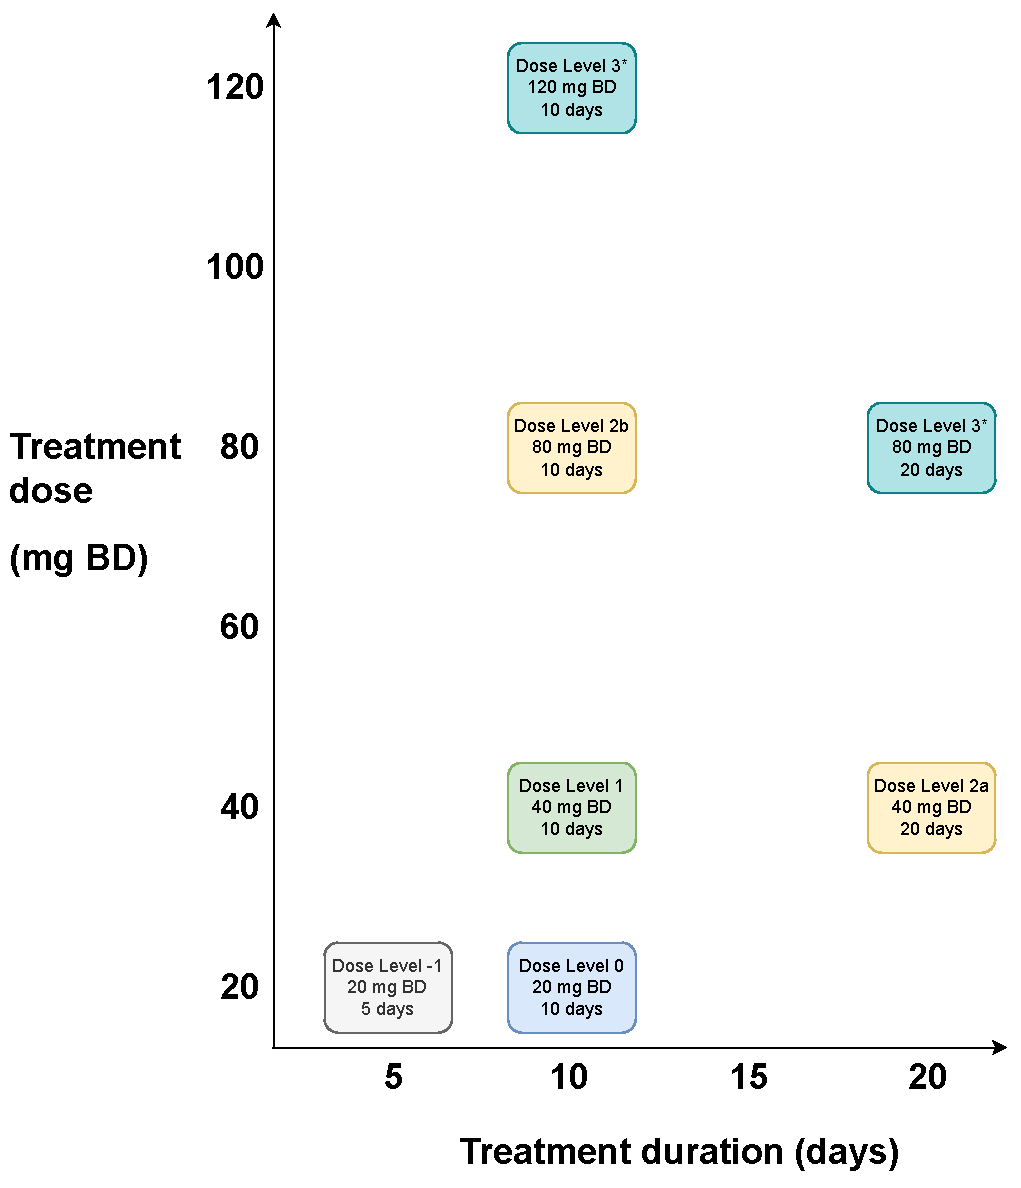
\includegraphics[width=\textwidth]{Adept-DoseCombos}
\end{figure}

It should be noted that our definition of orderings is assuming that total dose is the key driver in terms of probability of toxicity. If we were to relax this assumption it could be possible that dose-level 3 at 120 mg for 10 days (1200 mg total) could be considered less toxic than 2a 40 mg for 20 days (800 mg total). In this instance prolonged exposure to the treatment may be more toxic even though the total overall dose is lower. This would introduce a third ordering ($d_{-1} \rightarrow d_{0} \rightarrow d_{1} \rightarrow d_{2b} \rightarrow d_{3} \rightarrow d_{2a}$). However, since we are operating under the assumption that more overall dose increases probability of toxicity we will only consider the two orderings listed above. 

Traditionally, dose-finding trials for combinations would select dose levels to form a 'path' through the dose combination space such that each subsequent dose level was logically more toxic. This avoids the issue of partial ordering but means doses of interest or effective dose combinations may be missed or not investigated. Specifically, for ADePT-DDR this allows two 'paths' from dose level 1 extending to 2a and 2b. In terms of dose level 3 only one of the doses in that tier will be investigated, it was unclear as to which dose level would be best due to a lack of historical data. Even though dose level 3 is not yet specified in terms of modelling and simulations it was treated as singular dose. This was done as clinicians thought that it would be unlikely that we would reach these doses and that the probability of toxicity between them would be similar.  

Preliminary designs of the trial included only five dose levels and planned to use dose level 0 as the starting dose. During the trial design phase it was decided a new lower dose (dose level -1) would be introduced to allow for de-escalation if the initial dose was found to be too toxic. Dose escalation/de-escalation for subsequent cohorts would be determined from the two-stage PO-TITE-CRM. A two-stage design allows for escalation according to a pre-defined escalation scheme. The first stage dictates that if no DLT's are observed in the current cohort the dose allocated to the next cohort is the following dose in the escalation scheme. Dose levels continue to be incremented in this fashion until the first DLT is observed. In stage two, dose levels are determined by the PO-TITE-CRM.

Typically CRM designs begin by testing the first patient, or cohort, at the prior guess of TD or at a lower dose to be safe. However, clinicians may have safety concerns beginning the trial at higher dose levels as well as escalating to higher dose levels without testing lower ones. Investigators in ADePT-DDR expressed similar concerns as such a two-stage design was adopted. The escalation scheme used in stage one of ADePT-DDR will follow that of the first ordering ($d_{-1} \rightarrow d_{0} \rightarrow d_{1} \rightarrow d_{2a} \rightarrow d_{2b} \rightarrow d_{3}$). If patients in the first cohort (assigned to dose level 0) do not experience a DLT the next cohort will be allocated to dose level 1 and then if no DLTs are observed again the third cohort will be allocated to dose level 2a and so on and so forth. The dose escalation scheme was determined based on the prior probabilities of toxicity generated for each dose level.  

Information elicited from the investigators helped generate prior probabilities of toxicity for each dose level. They believed that dose level 2b would be the TD25 with 2a being less toxic. This was used in conjunction with the getprior function from the dfcrm R package \cite{cheungDfcrmDoseFindingContinual2019} which yielded priors of 0.012, 0.036, 0.084, 0.157, 0.25 and 0.355 for dose levels -1, 0, 1, 2a, 2b and 3 respectively. The half-width of the indifference interval was set at 0.05. The indifference interval is an interval in which the toxicity probability of the selected dose will eventually fall. Prior probabilities are also required for the plausibility of each model and even though the clinicians think that 2b will be more toxic than 2a there is no clear evidence and still a lot of uncertainty. As such it is sensible to assume a plausibility probability of 0.5 for each ordering, implying both orders are equally likely to be the true ordering of these dose levels. 

%-----------------------------------
%	SUBSECTION 3.2
%-----------------------------------
\subsection{The TITE component}
\label{adept:The-TITE-component}

The observation window for this trial will be up to a year post-treatment as the combination of radiotherapy with AZD6738 is anticipated to cause late-onset toxicity. The Acute DLT observation period is 12 weeks (84 days) post radiotherapy end with a minimum of 8 weeks (56 days) for the last patient of each cohort. However, patients will continuously be monitored for occurrence of DLT for at least 12 weeks (84 days), i.e. at least 12 weeks (84 days) from the end of radiotherapy. The full window will last for 52 weeks (365 days) post-treatment.

The TITE component incorporates a weighting contribution for each patient dependent on how long that patient has been evaluable in the study. This allows a patient to be evaluated once they have been observed for the minimum DLT period of 8 weeks (56 days). The weighting at this point is 60\% rising to 80\% at 12 weeks (84 days). A patient will not contribute fully to the model until they have completed 52 weeks (365 days) follow up (or have experienced a DLT at any stage in which case they will be weighted as a whole contribution). Linear weighting functions will be employed for any patient with a length of follow up between these three time points. One weight function to calculate weights between 8-12 weeks and another for weights between 12-52 weeks. For the weighting function $w(u;t_1, t_2, t_3)$ where $u$ is the time-to-toxicity of patient $j$ and $t_1, t_2, t_3$ is the time period with values 8, 12 and 52 respectively. Then for $t_1 \leq u \leq t_3$
\begin{equation}
w(u;t_1,t_2,t_3) = 0.6 + 0.2\frac{max(0, min(u, t_2) - t_1)}{t_2 - t_1} + 0.2\frac{max(0, u - t_2)}{t_3-t_2}.
\end{equation} 
All patients will have a minimum weight of 60\% as that is the prescribed weighting to the  minimum follow up period before dose escalation/de-escalation decisions can be made. For each additional week the patient is observed, without a DLT occurring, between weeks 8 and 12 their weighting increases by 5\%. Similarly for each week between 12 and 52 weeks, without a DLT, weighting increases by 0.5\%. Figure \ref{fig_adept:weight_function} illustrates the weight function and how the weight changes for patients dependent on how long they have been followed-up.   

\begin{figure}[h!]
	\centering
	\caption[Weight function across the follow-up period.]{Weights of patients who have not experienced a DLT across the observation window.}
	\label{fig_adept:weight_function}
	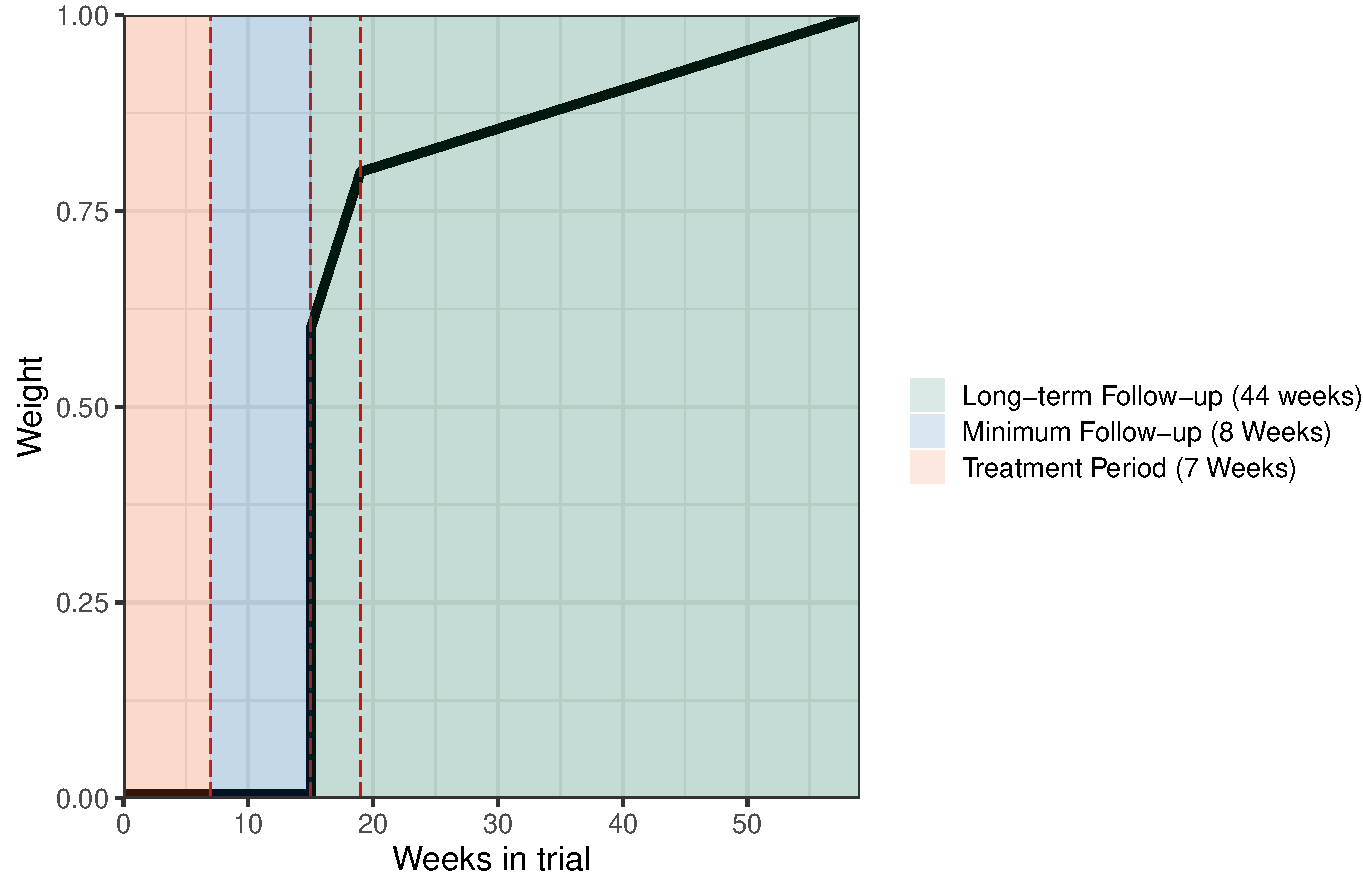
\includegraphics[width=\textwidth]{Adept-WeightFunction}
\end{figure}


The TITE-CRM originally presented by Cheung and Chappel \cite{cheungSequentialDesignsPhase2000} did not incorporate a minimum follow-up period and their design allowed for the continual recruitment of patients whenever they became available. There are some practical considerations which make this infeasible in ADePT-DDR. The model would need to be run each time a new patient entered the study which requires statistical input hence the introduction of cohorts. Clinicians may also have safety concerns if we see rapid recruitment at the start of the trial and the model keeps escalating so we impose a minimum follow-up period. Initially this was set at 12 weeks (at 80\% weighting) however, statisticians AP and PG  pointed out that dose escalation/de-escalation decisions would have to take place 19 weeks (7 weeks treatment and 12 weeks follow-up) after recruitment of the third patient in the cohort. Dependent on the recruitment rates this could extend the duration of the trial and negates the benefits of using a TITE design. The investigators also agreed this was too long and settled on lowering this period to 8 weeks (at 60\% weighting) whilst also including the original 12 week weighting of 80\%.


%-----------------------------------
%	SUBSECTION 3.3
%-----------------------------------
\subsection{Stopping rules}
\label{adept:Stopping-rules}

A practical modification was included to allow for early stopping of the trial if there is sufficient evidence that the TD has been reached. Sufficient evidence is achieved once 15 patients (five cohorts) have been treated at the same dose level and the model allocates that dose level again to a sixth cohort. This rule evolved from the original designs of the trial which involved 30 patients with a dose expansion cohort to ensure at least 15 patients were treated at the TD. 

Initial simulations highlighted the inadequacy of these design parameters as operating characteristics for various scenarios were poor, specifically in terms of correct TD selection. Clinicians explained the inclusion of the dose expansion cohort was to ensure the dose-finding aspect of the trial did not take a large amount of time whilst also allowing safety to be assessed at the TD. In order to ensure that a reasonable amount of patients would be treated at the TD, the trial would not take longer than necessary and operating characteristics improved, the sample size was increase and this rule was introduced.

A rule was also implemented to allow for early termination of the trial in the case of excess toxicity at the lowest dose. If the probability of DLT at the lowest dose is higher than 0.35 with a probability of 80\% and has been tested, the trials safety committee will be alerted and will recommend if the trial should be stopped. As the trial starts at dose level 0, which is not the lowest dose, it is possible for the trial to recommend terminating without ever allocating patients to the lowest dose level. As such it was decided early termination would only occur once at least 3 patients (1 cohort) have been allocated dose level -1. 

An approximate estimate of the variance was calculated using methodology presented by O'Quigley and Shen \cite{oquigleyContinualReassessmentMethod1996}. The observed information matrix is obtained by taking the second derivative of the likelihood (eq. \ref{eq_adept:likelihood}) which is then used to calculate the variance $v(\hat{\beta_j})$, for estimate $\beta_j$ which becomes more accurate with larger sample sizes. After each cohort, we sample from a normal distribution with parameters based on the estimate of $\beta_j$ and its variance. These samples are then plugged into our dose-toxicity model to ascertain the probability of toxicity at the lowest dose. The trial will be recommended to stop if it breaks the rule based on the criteria above. 

%-----------------------------------
%	SUBSECTION 3.4 
%-----------------------------------
\subsection{Example trial run}
\label{adept:toy} 

To demonstrate how the trial will run in practice we present an example trial run. Patients will be recruited in cohorts of three. After each cohort a dose will be recommended based on our design and the subsequent cohort of patients will be given that dose. This process is then repeated until the stopping rules are triggered. In our example here we observe no DLTs to begin with allowing us to follow the initial escalation scheme up to dose-level 3. At this point we begin to observe DLTs and thus begin to use the model to recommend dose-levels unti we stop for consensus. 

Table \ref{tab_adept:EstimatesExampleRun} shows model outputs after each cohorts specifically, the estimated probability of toxicity or DLT rate at each dose and the estimated posterior probability of each ordering. Order 1 refers to the order assuming 2b is more toxic than 2a and order 2 assumes 2a is more toxic than 2b. For the first initial four cohorts we see that there are no model outputs. This is because the model was not fit in these instances as no DLTs were observed. You can see the initial escalation scheme was followed. Meaning after cohort 1 received dose-level 0 cohort 2 received dose-level 1, cohort 3 received dose-level 2a and cohort 4 received dose-level 2b. 


\begin{table}[h!]
	
	\centering\begingroup\fontsize{9}{11}\selectfont
	\caption{\label{tab_adept:EstimatesExampleRun}Summary of model outputs for our example trial run.}
	\resizebox{\linewidth}{!}{
		\begin{tabular}{cccccccccccc}
			\toprule
			\multicolumn{3}{c}{ } & \multicolumn{6}{c}{Estimated DLT rate} & \multicolumn{2}{c}{Order prob} \\
			\cmidrule(l{3pt}r{3pt}){4-9} \cmidrule(l{3pt}r{3pt}){10-11}
			Cohort & Dose & DLT & -1 & 0 & 1 & 2a & 2b & 3 & 1 & 2 & Recommended Dose\\
			\midrule
			\cellcolor{gray!6}{1} & \cellcolor{gray!6}{0} & \cellcolor{gray!6}{0} & \cellcolor{gray!6}{} & \cellcolor{gray!6}{} & \cellcolor{gray!6}{} & \cellcolor{gray!6}{} & \cellcolor{gray!6}{} & \cellcolor{gray!6}{} & \cellcolor{gray!6}{} & \cellcolor{gray!6}{} & \cellcolor{gray!6}{1}\\
			2 & 1 & 0 &  &  &  &  &  &  &  &  & 2a\\
			\cellcolor{gray!6}{3} & \cellcolor{gray!6}{2a} & \cellcolor{gray!6}{0} & \cellcolor{gray!6}{} & \cellcolor{gray!6}{} & \cellcolor{gray!6}{} & \cellcolor{gray!6}{} & \cellcolor{gray!6}{} & \cellcolor{gray!6}{} & \cellcolor{gray!6}{} & \cellcolor{gray!6}{} & \cellcolor{gray!6}{2b}\\
			4 & 2b & 0 &  &  &  &  &  &  &  &  & 3\\
			\cellcolor{gray!6}{5} & \cellcolor{gray!6}{3} & \cellcolor{gray!6}{1} & \cellcolor{gray!6}{0} & \cellcolor{gray!6}{0} & \cellcolor{gray!6}{0.01} & \cellcolor{gray!6}{0.04} & \cellcolor{gray!6}{0.09} & \cellcolor{gray!6}{0.17} & \cellcolor{gray!6}{0.50} & \cellcolor{gray!6}{0.50} & \cellcolor{gray!6}{3}\\
			6 & 3 & 3 & 0.01 & 0.03 & 0.08 & 0.15 & 0.24 & 0.35 & 0.50 & 0.50 & 2b\\
			\cellcolor{gray!6}{7} & \cellcolor{gray!6}{2b} & \cellcolor{gray!6}{2} & \cellcolor{gray!6}{0.02} & \cellcolor{gray!6}{0.06} & \cellcolor{gray!6}{0.12} & \cellcolor{gray!6}{0.21} & \cellcolor{gray!6}{0.31} & \cellcolor{gray!6}{0.42} & \cellcolor{gray!6}{0.66} & \cellcolor{gray!6}{0.34} & \cellcolor{gray!6}{2a}\\
			8 & 2a & 0 & 0.02 & 0.05 & 0.10 & 0.18 & 0.28 & 0.39 & 0.73 & 0.27 & 2b\\
			\cellcolor{gray!6}{9} & \cellcolor{gray!6}{2b} & \cellcolor{gray!6}{0*} & \cellcolor{gray!6}{0.02} & \cellcolor{gray!6}{0.06} & \cellcolor{gray!6}{0.12} & \cellcolor{gray!6}{0.20} & \cellcolor{gray!6}{0.30} & \cellcolor{gray!6}{0.41} & \cellcolor{gray!6}{0.55} & \cellcolor{gray!6}{0.45} & \cellcolor{gray!6}{2a}\\
			10 & 2a & 0 & 0.02 & 0.04 & 0.10 & 0.18 & 0.27 & 0.38 & 0.62 & 0.38 & 2b\\
			\cellcolor{gray!6}{11} & \cellcolor{gray!6}{2b} & \cellcolor{gray!6}{0} & \cellcolor{gray!6}{0.01} & \cellcolor{gray!6}{0.03} & \cellcolor{gray!6}{0.08} & \cellcolor{gray!6}{0.15} & \cellcolor{gray!6}{0.24} & \cellcolor{gray!6}{0.34} & \cellcolor{gray!6}{0.57} & \cellcolor{gray!6}{0.43} & \cellcolor{gray!6}{2b}\\
			12 & 2b & 0 & 0.01 & 0.03 & 0.07 & 0.13 & 0.22 & 0.32 & 0.51 & 0.49 & 2b\\
			\bottomrule
			\multicolumn{12}{l}{\rule{0pt}{1em}\textsuperscript{*}  No DLTs in this cohort, but the previous cohort had a late onset DLT.}\\
	\end{tabular}}
	\endgroup{}
\end{table}

For cohort 5 we see that one patient in this cohort observed a DLT. Based on the model outputs in this scenario the estimated probability of toxicity at dose-level 3 is 0.17. As this is closes to our TD25 this becomes the dose that is recommended for cohort 6. We can also look at the estimates of probability for the orders, here both are at 0.5 indicating both orders are still equally likely. In cohort 6 a further three patients are recruited to dose-level 3 and we observe DLTs in all three patients. Overall, now there have been 4/6 DLTs at dose-level 3. Based on the model output here dose-level 2b with an estimated DLT rate of 0.24 is closest to the TD25 and is recommended for the next cohort. The posterior probability for the orders still indicate each order is equally likely. 

Now at cohort 7, patients are allocated to dose-level 2b. Here two DLTs are observed. The model recommends dose-level 2a. We can see the estimated probability of the orders suggests order 1 is more likely, which is indicative after having observed multiple toxicities at higher doses. Cohort 8 at dose-level 2a observes no toxicities which leads to the recommendation of going back to dose-level 2b. Here the estimated DLT rate here is 0.28 which is closer to the TD25 compared to any of the other doses. For the order probabilities we see again order 1 is still more likely. 

Cohort 9 recruits patients to dose-level 2b and observes no DLTs however, one patient from the previous cohort (cohort 8 dose-level 2a) has now experienced a late-onset DLT after the minimum follow-up period. Incorporating this new cohort data as well as the new DLT data for the previous cohort gives a model recommendation of going back to dose-level 2a. The exact estimated DLT rates for 2a and 2b were 0.2036 and 0.3037 respectively, 2a was narrowly the closest to dose-level 2b hence why it was recommended. The DLT at 2a also impacted the probabilities for each ordering. These still indicated 1 was more likely but they are much closer now.  

Going forward no more DLTs were observed and we can see the model keeps recommending dose-level 2b. Cohort 12 is the fifth cohort to treat patients at dose-level 2b, after observing no DLTs the model once again recommends dose-level 2b. This then triggers our consensus stopping rule as 15 patients have been treated a the same dose which is then recommended again. In this example dose-level 2b, with an estimated DLT rate of 0.22, is our TD25. 

Probabilities for the orders are now 0.51 and 0.49 for 1 and 2 respectively, meaning order 1 is slightly more likely. Overall dose-level 2a observed DLTs in 1/9 patients and dose-level 2b observed DLTs in 2/15 patients. In the data we observed there was no observable difference overall between the two doses. Earlier on in the trial the probabilities of the order fluctuated as more DLTs were observed. With potentially more data again this would change and keep updating. 

An additional point to consider is that at each dose decision or when the model is fit patients will have different weights based on the time spent in the trial without a DLT. For this example we assigned patients weights based on the weight function and the minimum follow-up period required. Figure \ref{fig_adept:toy_cohort_data} visualises the data that was used for the model output after each cohort. The shape of the points represent whether or not a patient had a DLT, the dose is represented by colour and the weight each patient had is represented by the transparency of the point. Later patients in a cohort tend to have less weight as they would have been recruited later, this is represented by the fainter points on the plot. For each subsequent cohort these points then become darker as patients gain more weight in the model after having been observed for a longer period of time.  Patients with DLTs are always at full weight. 

Figure \ref{fig_adept:toy_dose_data} shows an overall summary of the DLTs in each patient at each dose-level and shows how the doses change over time. One patient at dose-level 2a who had their DLT after the initial monitoring period which did not affect the recommendation for the next dose-level but for the cohorts thereafter. 

\begin{figure}[h!]
	\centering
	\caption{Plot of data included for each dose decision at each cohort.}
	\label{fig_adept:toy_cohort_data}
	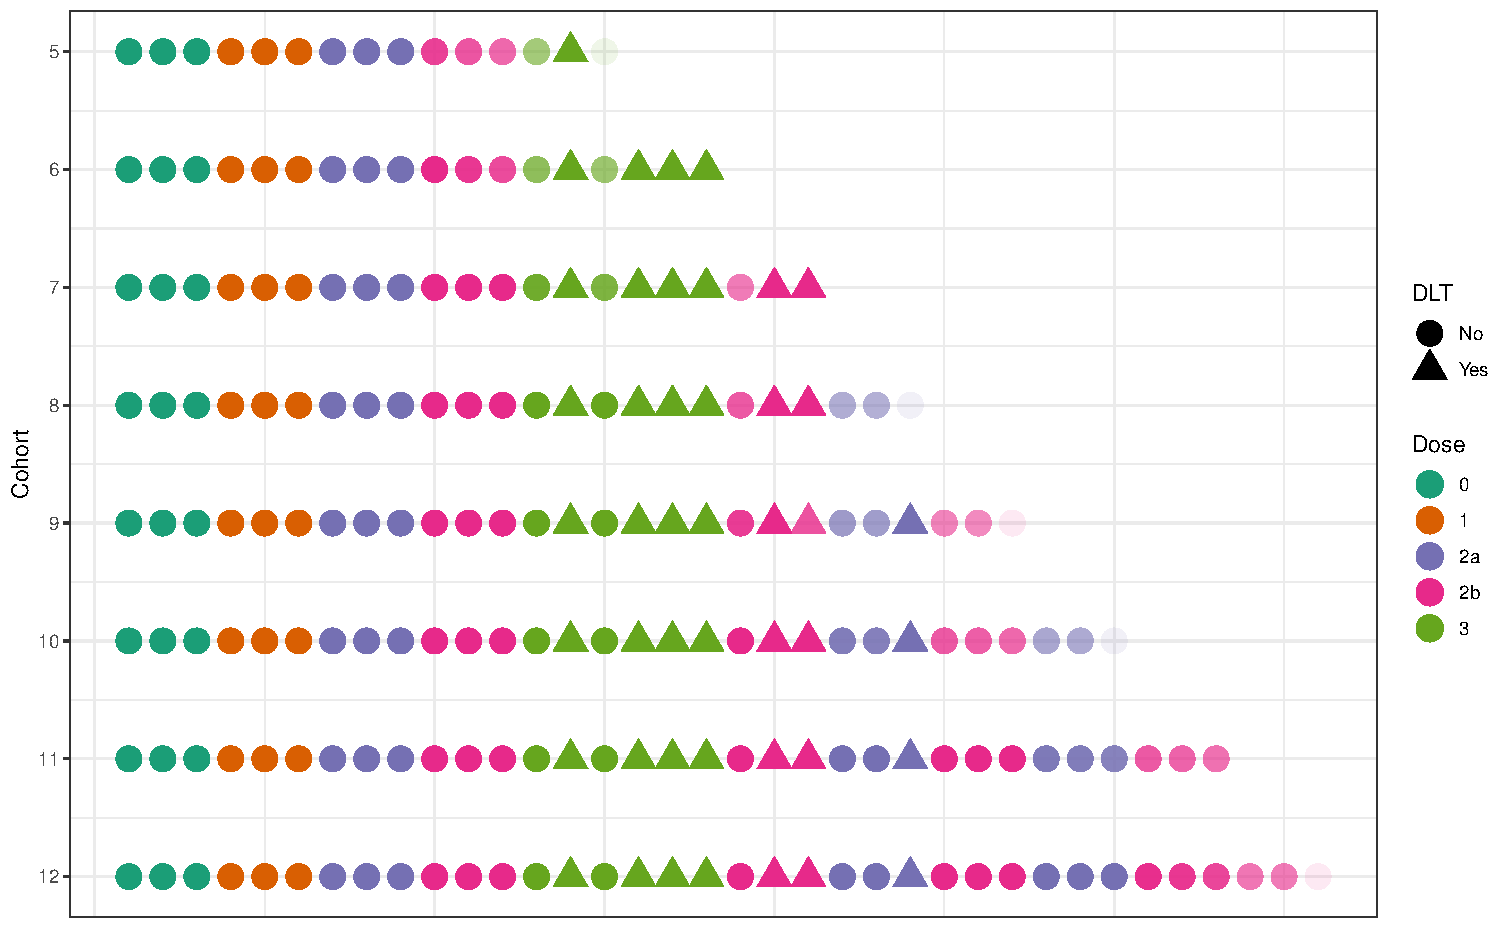
\includegraphics[width=\textwidth]{Adept-ToyCohortData}
\end{figure}


\begin{figure}[h!]
	\centering
	\caption{Plot of dose decisions throughout the example trial.}
	\label{fig_adept:toy_dose_data}
	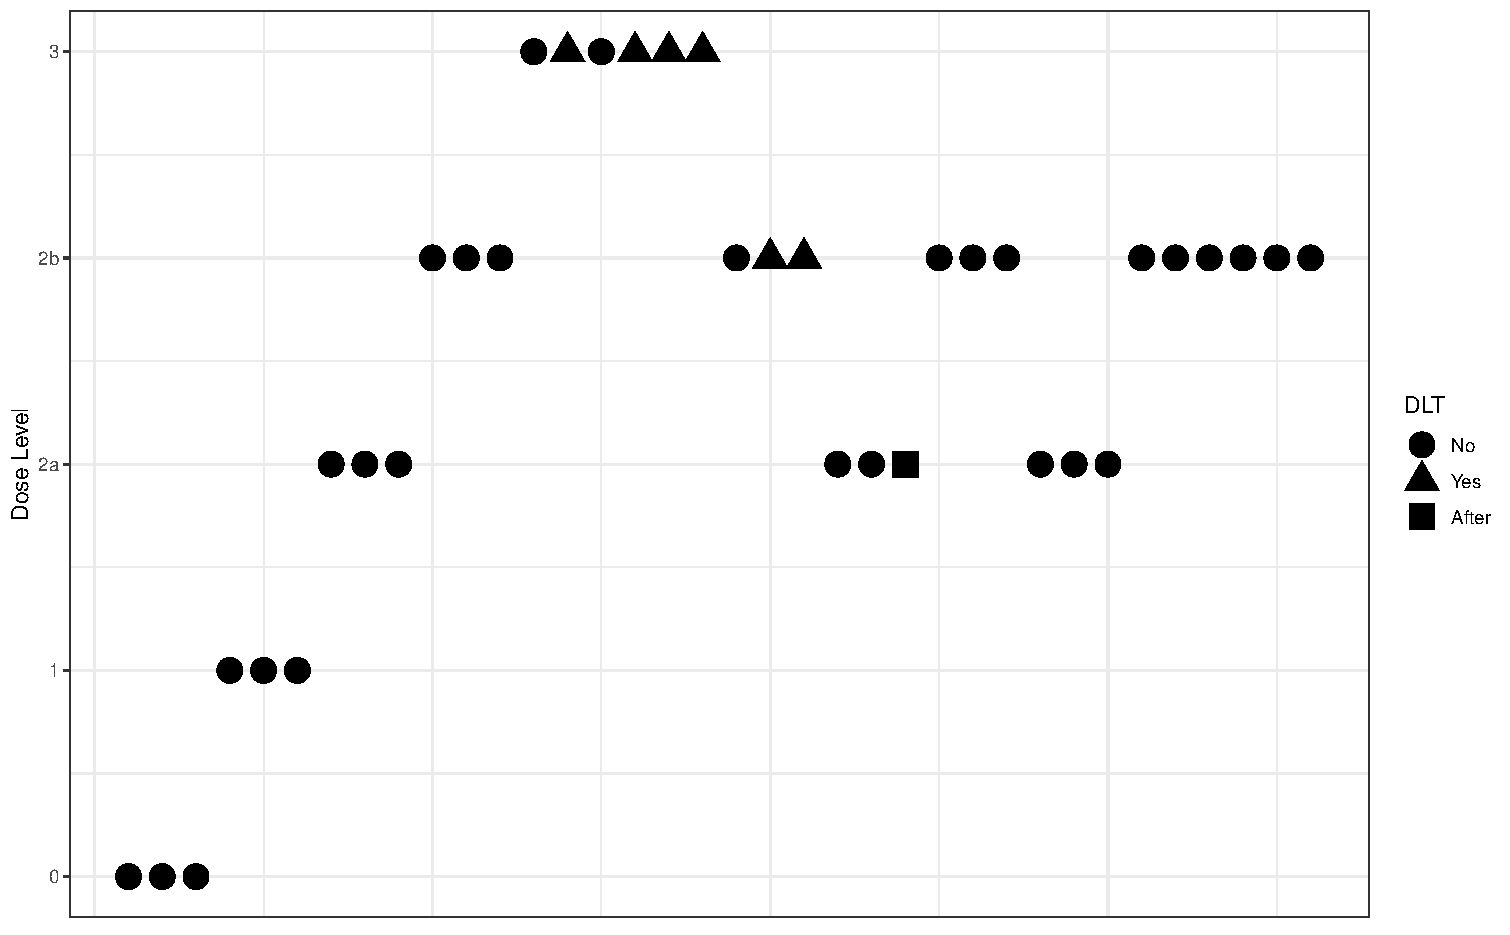
\includegraphics[width=\textwidth]{Adept-ToyDoseData}
\end{figure}

\newpage

%-----------------------------------
%	SUBSECTION 3.5 
%-----------------------------------
\subsection{Operating characteristics}
\label{adept:OCs} 

Simulations were continually utilised during the design process of the trial to assess how various changes impact the overall performance. These changes to design features such as the sample size, weight function and stopping rules helped inform decisions which led to the design specified in the previous section.  

Functions from pocrm package in R \cite{wagesPocrmRpackagePhase2013, wagesPocrmDoseFinding2019} were modified in order to perform simulations and conduct the trial. The majority of work involved integrating the TITE component and the stopping rules into the code. In standard CRM designs a binary outcome for toxicity is generated for each patient based on a pre-specified true DLT rates for the dose they are assigned. Adding the TITE component means the time the toxicity occurs also has to be generated, the simulation must also track this time and incorporate this information into the PO-TITE-CRM model when it needs to make dose allocation decisions for the next cohort. We defined multiple scenarios to reflect various real life possibilities in order to assess the design's performance.  

Standard scenarios to run involve adjusting the true DLT rates to reflect each dose being the TD25. For each of these we calculate the probability of selecting each dose as the TD25. It would be expected the dose with the highest probability of being selected has its true DLT rate set at 25\% to match the target rate. A high probability of selection for the correct dose implies the design works well in the specified scenario. Additional characteristics such as the average number of patients at each dose level are also investigated. This can be used to look at how many patients may potentially be allocated to a toxic dose. It is also necessary to consider performance when all doses are too toxic, here we would want the design to recommend stopping early. Usually the true DLT rates used to define these scenarios abide by the monotonicity assumption. Due to the partial ordering we consider scenarios in which the true DLT rates follow both orders. However, as ADePT-DDR only has two orders we explored all scenarios for each ordering.

We simulated 10000 trials for each scenario using the finalised design detailed in section \ref{adept:PO-TITE-CRM-in-Adept}. Simulations were based on the assumption that the trial would recruit one patient per month. The occurrence of DLT's were randomly generated for patients in each cohort using a Bernoulli distribution with the probability set at the true DLT rate for the cohorts assigned dose level in the specific scenario. For patients who had a DLT occur, the time at which the DLT occurred was randomly generated using a uniform distribution which spanned the start of treatment to the end of follow-up. The simulations presented in Tables \ref{tab_adept:OCorder1} and \ref{tab_adept:OCorder2} took approximately 5 hours and 53 minutes to run. It is recommended by Morris et al. \cite{morrisUsingSimulationStudies2019} to detail the Monte Carlo standard error in order to quantify the simulations uncertainty. In the case of a 50\% selection probability the Monte Carlo standard error estimated by 10000 simulations is $\sqrt{0.5 \times 0.5/10000} = 0.5\%$. This implies that differences of 1\% can be deemed as significant. 

Table \ref{tab_adept:OCorder1} details simulations for eight scenarios to test the performance of the PO-TITE-CRM design using true DLT rates which reflect the first ordering. We analyse scenarios where each dose is the TD25 (scenarios 1-6) and when all doses are too toxic (scenario 8). Additionally, we also investigate performance under conditions where the probability of DLT is fairly similar between doses (scenario 7). This is a notoriously difficult circumstance for CRM designs to deal with as the limited number of patients and events at each dose make it hard to accurately estimate toxicity probabilities if they are similar. Simulation results for ordering 2 are shown in Table \ref{tab_adept:OCorder2} where dose level 2a is considered more toxic than 2b. This is achieved by altering the true DLT rates so 2b has a lower probability of DLT compared to 2a. 

Ideally we want the probability of selection for the dose allocated at TD25 to be as high as possible and greater than other dose levels. For scenarios 1-7 the TD25 is highlighted in bold along with results from the simulations. However, for scenario 8 where all doses are too toxic we expect the trial to terminate early, here 'stop' should be selected and its associated probability of stopping is shown in bold. 

\begin{table}[h!] % OC for order 1 
	
	\caption[Operating Characteristics for ordering 1.]{\label{tab_adept:OCorder1} Operating Characteristics of the two-stage PO-TITE-CRM (with true DLT rates that imply 2b is more toxic than 2a) based on 10000 simulated trials. Definitions: DLT: Dose-limiting toxicity. P(select):
		Probability of selecting a dose as the TD25.}
	\centering
	\begin{singlespace}
		\resizebox{\linewidth}{!}{
			\begin{tabular}[t]{ccccccccc}
				\toprule
				\multicolumn{2}{c}{ } & \multicolumn{6}{c}{Dose Levels} \\
				\cmidrule(l{3pt}r{3pt}){3-8}
				&  & -1 & 0 & 1 & 2a & 2b & 3 & Stop\\
				\midrule
				Scenario & Prior DLT & 0.01 & 0.04 & 0.08 & 0.16 & 0.25 & 0.35 & \\
				\cmidrule{1-9}
				\rowcolor{gray!6}   & True DLT rate & 0.25 & 0.4 & 0.45 & 0.5 & 0.55 & 0.6 & \\
				
				\rowcolor{gray!6}   & P(select) & \textbf{0.68} & 0.18 & 0.05 & 0.01 & 0 & 0 & 0.08\\
				
				\rowcolor{gray!6}   & \% of patients & 39 & 32 & 20 & 6 & 3 & 0 & \\
				
				\rowcolor{gray!6}  \multirow{-4}{*}{\centering\arraybackslash 1: TD25 @-1} & Mean number of patients & 10.17 & 8.46 & 5.33 & 1.67 & 0.69 & 0.07 & \\
				\cmidrule{1-9}
				& True DLT rate & 0.12 & 0.25 & 0.4 & 0.45 & 0.5 & 0.55 & \\
				
				& P(select) & 0.23 & \textbf{0.51} & 0.2 & 0.03 & 0.02 & 0 & 0.01\\
				
				& \% of patients & 17 & 35 & 29 & 11 & 6 & 1 & \\
				
				\multirow{-4}{*}{\centering\arraybackslash 2: TD25 @0} & Mean number of patients & 5.24 & 10.48 & 8.75 & 3.4 & 1.83 & 0.26 & \\
				\cmidrule{1-9}
				\rowcolor{gray!6}   & True DLT rate & 0.09 & 0.12 & 0.25 & 0.4 & 0.45 & 0.5 & \\
				
				\rowcolor{gray!6}   & P(select) & 0.02 & 0.2 & \textbf{0.55} & 0.14 & 0.09 & 0.01 & $<$0.01\\
				
				\rowcolor{gray!6}   & \% of patients & 4 & 20 & 34 & 23 & 16 & 3 & \\
				
				\rowcolor{gray!6}  \multirow{-4}{*}{\centering\arraybackslash 3: TD25 @1} & Mean number of patients & 1.22 & 6.41 & 10.97 & 7.23 & 5.14 & 1.02 & \\
				\cmidrule{1-9}
				& True DLT rate & 0.06 & 0.09 & 0.12 & 0.25 & 0.4 & 0.45 & \\
				
				& P(select) & 0 & 0.02 & 0.22 & \textbf{0.48} & 0.23 & 0.05 & $<$0.01\\
				
				& \% of patients & 1 & 12 & 20 & 31 & 25 & 11 & \\
				
				\multirow{-4}{*}{\centering\arraybackslash 4: TD25 @2a} & Mean number of patients & 0.47 & 3.88 & 6.74 & 10.43 & 8.2 & 3.5 & \\
				\cmidrule{1-9}
				\rowcolor{gray!6}   & True DLT rate & 0.03 & 0.06 & 0.09 & 0.12 & 0.25 & 0.4 & \\
				
				\rowcolor{gray!6}   & P(select) & 0 & 0 & 0.02 & 0.3 & \textbf{0.43} & 0.25 & 0\\
				
				\rowcolor{gray!6}   & \% of patients & 1 & 10 & 12 & 24 & 28 & 25 & \\
				
				\rowcolor{gray!6}  \multirow{-4}{*}{\centering\arraybackslash 5: TD25 @2b} & Mean number of patients & 0.25 & 3.36 & 4.15 & 8.17 & 9.33 & 8.33 & \\
				\cmidrule{1-9}
				& True DLT rate & 0.01 & 0.03 & 0.06 & 0.09 & 0.12 & 0.25 & \\
				
				& P(select) & 0 & 0 & 0 & 0.09 & 0.13 & \textbf{0.78} & 0\\
				
				& \% of patients & 0 & 10 & 11 & 18 & 18 & 42 & \\
				
				\multirow{-4}{*}{\centering\arraybackslash 6: TD25 @3} & Mean number of patients & 0.1 & 3.13 & 3.49 & 5.46 & 5.6 & 13.14 & \\
				\cmidrule{1-9}
				\rowcolor{gray!6}   & True DLT rate & 0.05 & 0.1 & 0.15 & 0.2 & 0.25 & 0.3 & \\
				
				\rowcolor{gray!6}   & P(select) & 0 & 0.03 & 0.12 & 0.31 & \textbf{0.28} & 0.26 & $<$0.01\\
				
				\rowcolor{gray!6}   & \% of patients & 2 & 13 & 18 & 26 & 23 & 19 & \\
				
				\rowcolor{gray!6}  \multirow{-4}{*}{\centering\arraybackslash 7: Equal steps in DLT rate} & Mean number of patients & 0.55 & 4.03 & 5.72 & 8.32 & 7.15 & 5.96 & \\
				\cmidrule{1-9}
				& True DLT rate & 0.5 & 0.6 & 0.65 & 0.7 & 0.75 & 0.8 & \\
				
				& P(select) & 0.26 & 0 & 0 & 0 & 0 & 0 & \textbf{0.74}\\
				
				& \% of patients & 56 & 26 & 15 & 2 & 0 & 0 & \\
				
				\multirow{-4}{*}{\centering\arraybackslash 8: All  toxic} & Mean number of patients & 9.05 & 4.27 & 2.4 & 0.37 & 0.04 & 0 & \\
				\bottomrule
			\end{tabular}
		}
	\end{singlespace}
\end{table}

\begin{table}[h!] % OC for order 2
	
	\caption[Operating Characteristics for ordering 2.]{\label{tab_adept:OCorder2}  Operating Characteristics of the two-stage PO-TITE-CRM (with true DLT rates that imply 2a is more toxic than 2b) based on 10000 simulated trials. Definitions: DLT: Dose-limiting toxicity. P(select): Probability of selecting a dose as the TD25.}
	\centering
	\begin{singlespace}
		\resizebox{\linewidth}{!}{
			\begin{tabular}[t]{ccccccccc}
				\toprule
				\multicolumn{2}{c}{ } & \multicolumn{6}{c}{Dose Levels} \\
				\cmidrule(l{3pt}r{3pt}){3-8}
				&  & -1 & 0 & 1 & 2a & 2b & 3 & Stop\\
				\midrule
				Scenario & Prior DLT & 0.01 & 0.04 & 0.08 & 0.16 & 0.25 & 0.35 & \\
				\cmidrule{1-9}
				\rowcolor{gray!6}   & True DLT rate & 0.25 & 0.4 & 0.45 & 0.55 & 0.5 & 0.6 & \\
				
				\rowcolor{gray!6}   & P(select) & \textbf{0.67} & 0.19 & 0.05 & 0 & 0.01 & 0 & 0.08\\
				
				\rowcolor{gray!6}   & \% of patients & 39 & 32 & 20 & 6 & 3 & 0 & \\
				
				\rowcolor{gray!6}  \multirow{-4}{*}{\centering\arraybackslash 9: TD25 @-1} & Mean number of patients & 10.19 & 8.43 & 5.27 & 1.6 & 0.68 & 0.07 & \\
				\cmidrule{1-9}
				& True DLT rate & 0.12 & 0.25 & 0.4 & 0.5 & 0.45 & 0.55 & \\
				
				& P(select) & 0.23 & \textbf{0.52} & 0.2 & 0.02 & 0.02 & 0 & 0.01\\
				
				& \% of patients & 18 & 36 & 29 & 11 & 6 & 1 & \\
				
				\multirow{-4}{*}{\centering\arraybackslash 10: TD25 @0} & Mean number of patients & 5.24 & 10.64 & 8.82 & 3.16 & 1.85 & 0.24 & \\
				\cmidrule{1-9}
				\rowcolor{gray!6}   & True DLT rate & 0.09 & 0.12 & 0.25 & 0.45 & 0.4 & 0.5 & \\
				
				\rowcolor{gray!6}   & P(select) & 0.02 & 0.2 & \textbf{0.55} & 0.09 & 0.14 & 0.01 & $<$0.01\\
				
				\rowcolor{gray!6}   & \% of patients & 4 & 20 & 34 & 21 & 17 & 3 & \\
				
				\rowcolor{gray!6}  \multirow{-4}{*}{\centering\arraybackslash 11: TD25 @1} & Mean number of patients & 1.16 & 6.43 & 11.07 & 6.83 & 5.6 & 1.07 & \\
				\cmidrule{1-9}
				& True DLT rate & 0.06 & 0.09 & 0.12 & 0.25 & 0.15 & 0.45 & \\
				
				& P(select) & 0 & 0.01 & 0.08 & \textbf{0.44} & 0.33 & 0.14 & $<$0.01\\
				
				& \% of patients & 1 & 11 & 16 & 30 & 24 & 18 & \\
				
				\multirow{-4}{*}{\centering\arraybackslash 12: TD25 @2a} & Mean number of patients & 0.48 & 3.78 & 5.24 & 10.1 & 7.9 & 6.07 & \\
				\cmidrule{1-9}
				\rowcolor{gray!6}   & True DLT rate & 0.03 & 0.06 & 0.09 & 0.35 & 0.25 & 0.4 & \\
				
				\rowcolor{gray!6}   & P(select) & 0 & 0 & 0.15 & 0.31 & \textbf{0.43} & 0.11 & 0\\
				
				\rowcolor{gray!6}   & \% of patients & 1 & 11 & 18 & 30 & 28 & 14 & \\
				
				\rowcolor{gray!6}  \multirow{-4}{*}{\centering\arraybackslash 13: TD25 @2b} & Mean number of patients & 0.25 & 3.5 & 5.9 & 9.82 & 9.14 & 4.54 & \\
				\cmidrule{1-9}
				& True DLT rate & 0.01 & 0.03 & 0.06 & 0.12 & 0.09 & 0.25 & \\
				
				& P(select) & 0 & 0 & 0 & 0.13 & 0.09 & \textbf{0.78} & 0\\
				
				& \% of patients & 0 & 10 & 11 & 19 & 16 & 43 & \\
				
				\multirow{-4}{*}{\centering\arraybackslash 14: TD25 @3} & Mean number of patients & 0.1 & 3.13 & 3.51 & 5.88 & 5.06 & 13.13 & \\
				\cmidrule{1-9}
				\rowcolor{gray!6}   & True DLT rate & 0.05 & 0.1 & 0.15 & 0.25 & 0.2 & 0.3 & \\
				
				\rowcolor{gray!6}   & P(select) & 0 & 0.02 & 0.12 & \textbf{0.32} & 0.27 & 0.26 & $<$0.01\\
				
				\rowcolor{gray!6}   & \% of patients & 2 & 13 & 19 & 27 & 22 & 18 & \\
				
				\rowcolor{gray!6}  \multirow{-4}{*}{\centering\arraybackslash 15: Equal steps in DLT rate} & Mean number of patients & 0.54 & 4.02 & 5.93 & 8.56 & 6.89 & 5.75 & \\
				\cmidrule{1-9}
				& True DLT rate & 0.5 & 0.6 & 0.65 & 0.75 & 0.7 & 0.8 & \\
				
				& P(select) & 0.27 & 0 & 0 & 0 & 0 & 0 & \textbf{0.73}\\
				
				& \% of patients & 56 & 27 & 15 & 2 & 0 & 0 & \\
				
				\multirow{-4}{*}{\centering\arraybackslash 16: All  toxic} & Mean number of patients & 9.01 & 4.28 & 2.39 & 0.38 & 0.05 & 0 & \\
				\bottomrule
		\end{tabular}}
	\end{singlespace}
\end{table}

In scenarios 1 - 6 (Table \ref{tab_adept:OCorder1}), this design correctly selects the TD25 with probabilities between 43\% and 78\%, under the assumption 2b is more toxic than 2a. Likewise, for the ordering where 2a is more toxic than 2b, scenarios 9-14 (Table \ref{tab_adept:OCorder2}) have probabilities between 43\% and 78\% of correctly selecting the TD25. Correct selection probabilities are generally higher when the TD25 is at the first and last dose levels compared to dose levels 2a and 2b. However, these dose levels are still chosen with the highest probability as the TD25 in their given scenarios. For scenarios 7 and 15, the probabilities of toxicity are equally spaced, approximately 5\% apart. This is a relatively difficult scenario for dose-finding studies to handle. The probability of selecting the TD25 is 28\% and 32\% for orderings 1 and 2 respectively and even if the performance is poor the correct dose is still likely to be selected. In scenarios 8 and 16, where all the doses are too toxic, the design very seldom allocates patients higher than the first three doses and there is a high chance (74\% and 73\% respectively) that the trial will recommend early stopping.

Additionally, we assess designs based on how doses are allocated to patients. Designs may correctly select the TD however, this could be undesirable and unethical if the majority of patients are over-dosed at the more toxic dose levels. The average number and the percentage of patients at each dose level, for each scenario, is recorded in Tables \ref{tab_adept:OCorder1} and \ref{tab_adept:OCorder2}. 

The percentage of patients treated at the TD25 ranges between 23\% and 43\% for each scenario under both orderings. The design also allocates the most patients on average to the TD25 apart from in scenario 7. In this case more patients were allocated to the next lowest dose, we have already discussed the difficulties of this scenario so this characteristic is not too concerning. The mean number of patients recruited for scenarios 1-6 is 26, 30, 32, 33, 34 and 31 respectively. Similarly for scenarios 9-14 its 26, 30, 32, 34, 33 and 31. Even though we allow for up to 60 patients the majority of trials terminate early based on the pre-defined rules for selecting the TD25. This information is presented in Table \ref{tab_adept:SummaryN_POTITESims} which also shows how often the max sample size is reached from the 10000 trials for each scenario. 

\begin{table}[h!]
	
	\caption{\label{tab_adept:SummaryN_POTITESims}Summary of simulated patient numbers for each scenario.}
	\centering
	\resizebox{\linewidth}{!}{
		\begin{tabular}[t]{cccc}
			\toprule
				Scenario & Max no. of patients & \% max reached & Mean no. of patients\\
				\midrule
				\cellcolor{gray!6}{1: TD25 @-1} & \cellcolor{gray!6}{60} & \cellcolor{gray!6}{0.21} & \cellcolor{gray!6}{26.38}\\
				2: TD25 @0 & 60 & 0.08 & 29.97\\
				\cellcolor{gray!6}{3: TD25 @1} & \cellcolor{gray!6}{60} & \cellcolor{gray!6}{0.05} & \cellcolor{gray!6}{32.01}\\
				4: TD25 @2a & 60 & 0.12 & 33.22\\
				\cellcolor{gray!6}{5: TD25 @2b} & \cellcolor{gray!6}{60} & \cellcolor{gray!6}{0.06} & \cellcolor{gray!6}{33.60}\\
				6: TD25 @3 & 60 & 0.02 & 30.92\\
				\cellcolor{gray!6}{7: Equal steps} & \cellcolor{gray!6}{60} & \cellcolor{gray!6}{0.01} & \cellcolor{gray!6}{31.74}\\
				8: All toxic & 54 & 0.01 & 16.14\\
				\cellcolor{gray!6}{9: TD25 @-1} & \cellcolor{gray!6}{60} & \cellcolor{gray!6}{0.17} & \cellcolor{gray!6}{26.24}\\
				10: TD25 @0 & 60 & 0.11 & 29.95\\
				\cellcolor{gray!6}{11: TD25 @1} & \cellcolor{gray!6}{60} & \cellcolor{gray!6}{0.06} & \cellcolor{gray!6}{32.15}\\
				12: TD25 @2a & 60 & 0.07 & 33.56\\
				\cellcolor{gray!6}{13: TD25 @2b} & \cellcolor{gray!6}{60} & \cellcolor{gray!6}{0.03} & \cellcolor{gray!6}{33.16}\\
				14: TD25 @3 & 60 & 0.08 & 30.81\\
				\cellcolor{gray!6}{15: Equal steps} & \cellcolor{gray!6}{60} & \cellcolor{gray!6}{0.02} & \cellcolor{gray!6}{31.69}\\
				16: All toxic & 51 & 0.01 & 16.11\\
			\bottomrule
	\end{tabular}}
\end{table}


Overall, the simulation results show the specification of this design performs relatively well in a number of scenarios. We have shown there is a high probability of the trial stopping early if all dose-levels are too toxic. We have also shown the design behaves in an appropriate manner when there is a lack of disparity between dose-levels in terms of toxicity. Finally, we have demonstrated that regardless of the ordering we observe the PO-TITE-CRM has a high probability of selecting the correct dose. There are a number of limitations to the operating characteristics presented here which are due to the specification of the simulations and trial design. Section \ref{adept:Exploring-other-designs} explores and discusses these limitations in more detail.


%----------------------------------------------------------------------------------------
%	SECTION 4
%-------------------------.

\section{Exploring other designs}  
\label{adept:Exploring-other-designs}

The operating characteristics presented in section \ref{adept:OCs} provide an insight into how the trial design operates and its effectiveness at selecting the TD25. However, several factors impact the results seen here. These factors can be grouped into two main categories, limitations with the simulations performed or the trial design.

To simulate various scenarios the true DLT rates are adjusted to reflect the TD25 being at different dose levels. There is no formal process to select these values as such their selection is fairly arbitrary. We set one dose level as the TD25 with lower and higher dose levels set at lower and higher DLT rates respectively. Figure \ref{fig_adept:dlt_rates} illustrates the dose levels for scenarios in Table \ref{tab_adept:OCorder1} where dose level 2b is more toxic than 2a. The DLT rates cover some possible scenarios and account for a range of plausible values. However, these true DLT rates may not accurately reflect what we observe once the trial begins. Also, the relationship between the rates and the dose levels may not be similar to what we use in the simulations. Multiple other scenarios could be investigated but it would still be impossible to account for all possible variations which may occur. Hence when evaluating the performance of a design it is important to note the scenario in which it is being evaluated and whether or not the design performs as expected and to an adequate level. For ADePT-DDR, the design produces reasonable operating characteristics under each scenario. 

\begin{figure}[h!]
	\centering
	\caption[Illustration of true DLT rates used in simulations.]{True DLT rates used for each of the scenarios where dose level 2b is more toxic than 2a. The dotted red line represents the target dlt rate of 25\% (TD25).}
	\label{fig_adept:dlt_rates}
	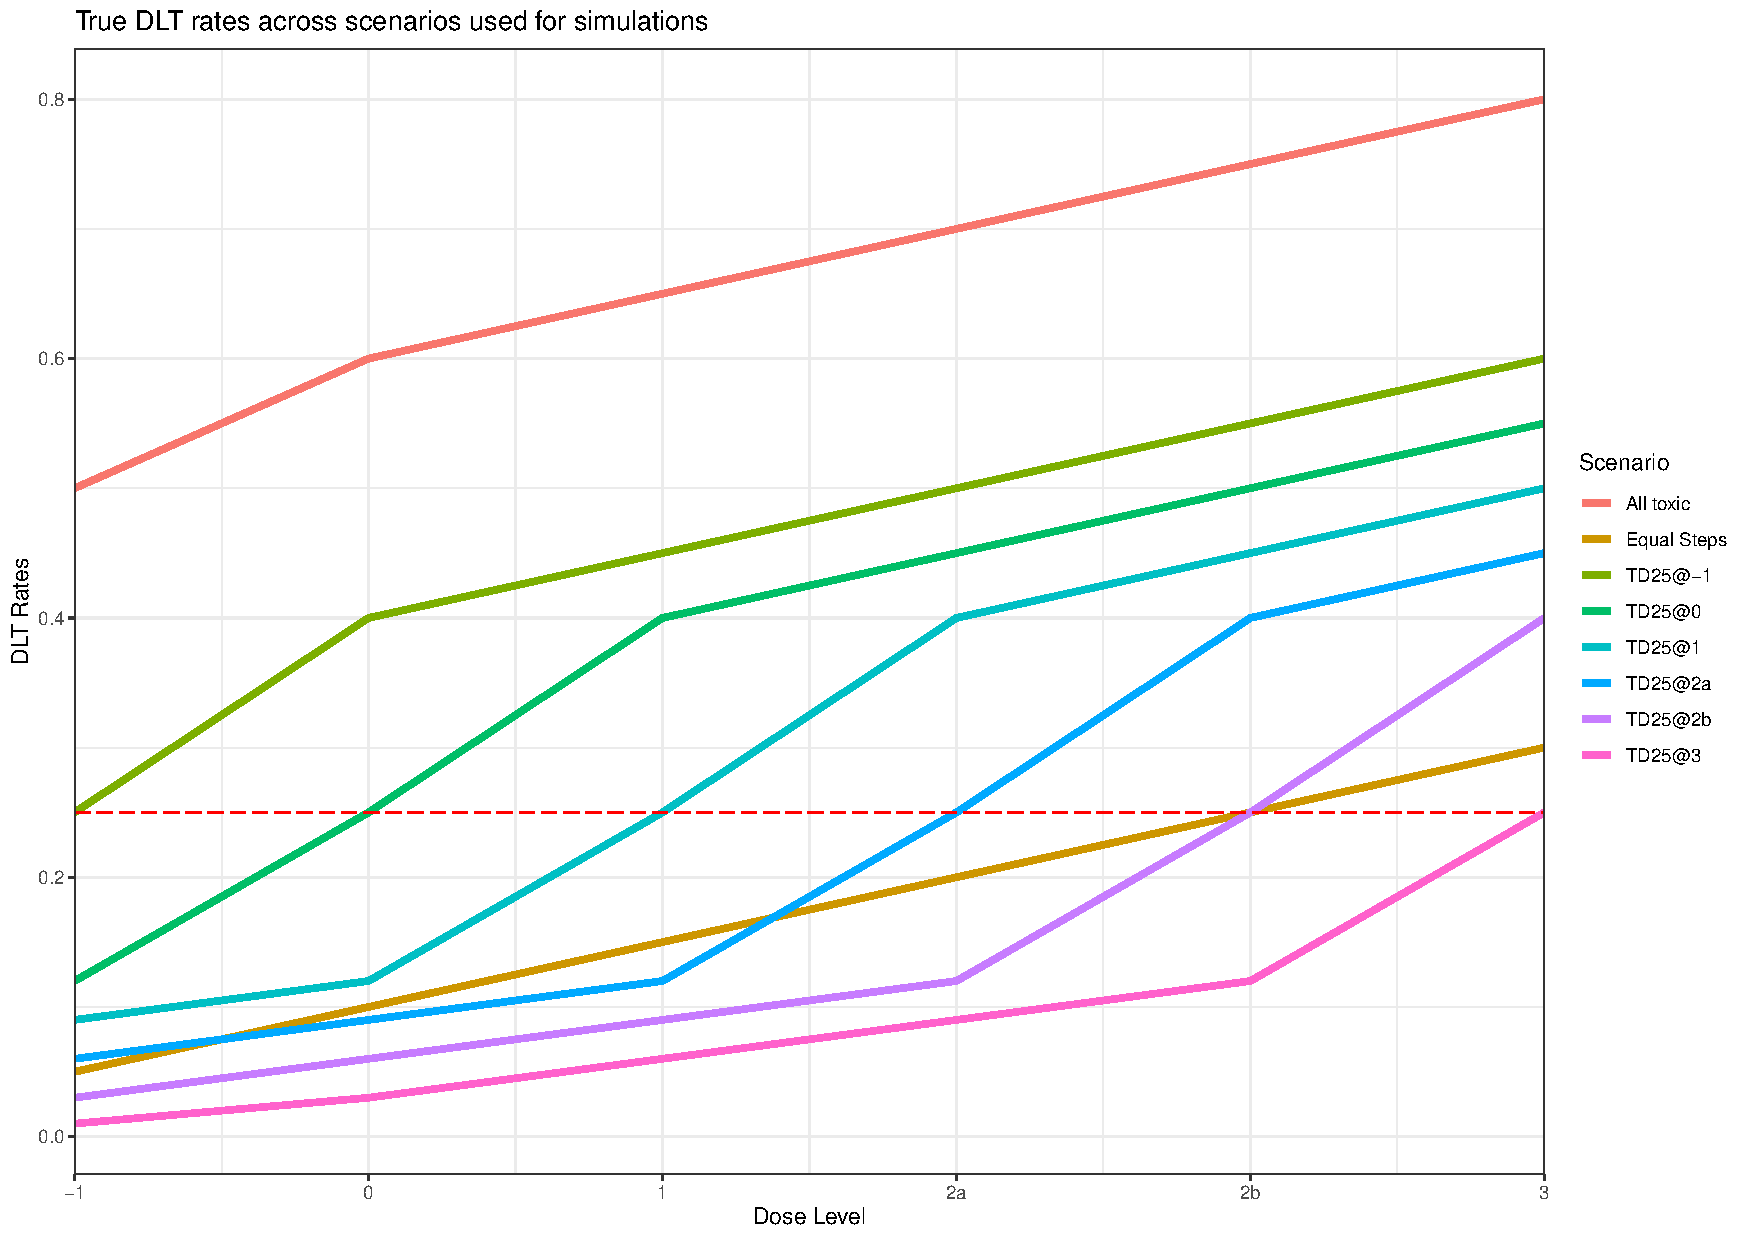
\includegraphics[width=\textwidth]{Adept-DLTRates}
\end{figure}
 
The original methodological papers by Wages et al. \cite{wagesUsingTimetoeventContinual2013,wagesContinualReassessmentMethod2011} only provide simulations for their examples using true DLT rates that are monotonically increasing which represented one of their possible orderings. Initially, in ADePT-DDR we followed suit and only produced simulations under a monotonically increasing DLT rate (order where 2b is more toxic than 2a, Table \ref{tab_adept:OCorder1}). However, as we are unclear on the ordering of 2a and 2b there is a possibility that 2b is less toxic. So those initial simulations would not provide an accurate assessment of the design in that circumstance. This was the main motivation for running scenarios in Table \ref{tab_adept:OCorder2}, in which we see the design performs at a similar level regardless of the partial ordering. ADePT-DDR is a simple case of partial ordering as there are only two possible orderings and six dose-levels. For trials with higher numbers of orderings or dose-levels the number of scenarios that would have to be evaluated would increase which may be infeasible. Here it may be more beneficial to choose a handful of scenarios from multiple different orderings to cover a wider range of possible outcomes for the trial to assess the design. 

There are various features in this trial design that impact how it performs. The partial ordering caused by dose levels 2a and 2b adds complexity to design. If one of these dose-levels were to be removed or a normal ordering was assumed a standard TITE-CRM design could be used instead. However, this would take away from what the trial is trying to discover. This trial also has a long follow-up period due to potential late-onset toxicities and in turn, will have a long duration. The TITE component will allow for the duration to be a lot shorter than it would be otherwise. TITE-CRM designs allow for patients to be recruited sequentially and allocated a dose based on available information from patients already in the trial. The design for ADePT-DDR uses cohorts of three and a minimum follow-up period. The dose-escalation decisions will only be made every third patient after a specific amount of time. This is done for safety and practicality reasons but means that some patients may not be able to enter the trial and it also loses some of the benefits of the TITE-CRM. We also have a sample size of 60 patients but include a stopping rule for when a consensus is reached which means we often do not recruit the maximum sample size. Further simulations were produced to investigate how these features affected the trial. Tables \ref{tab_adept:Design_Comparison1} and \ref{tab_adept:Design_Comparison2} compares selection probabilities as well as duration measured in months from the ADePT-DDR trial design with five alternative designs based on the two different orderings. Figures \ref{fig_adept:sims_order1} and \ref{fig_adept:sims_order2} visualise the result from each of these tables respectively. 10000 trials were simulated for each scenario which took 62 hours and 22 minutes to complete.  
 
\begin{enumerate}
	\item TITE-CRM design. This design assumes that partial ordering does not exist and that dose-level 2b is more toxic than 2a. A TITE-CRM is used instead of a PO-TITE-CRM. All other stopping rules and details remain the same. 
	\item PO (Partial Ordering design). This design removes the TITE component and uses a PO-CRM as detailed by \cite{wagesContinualReassessmentMethod2011}. This requires the removal of the minimum follow-up period so all dose allocation decisions are made once all 3 patients in a cohort have been observed for the full follow-up period of one year. All other stopping rules and details remain the same. 
	\item N = 30. This design uses a fixed sample size of 30 patients and removes the stopping rule for reaching consensus. The analysis is still conducted using the PO-TITE-CRM. All other stopping rules and details remain the same. 
	\item N = 60. This design uses a fixed sample size of 60 patients and removes the stopping rule for reaching consensus. The analysis is still conducted using the PO-TITE-CRM. All other stopping rules and details remain the same. 
	\item CS = 1. This design uses a cohort size (CS) of one. All other stopping rules remain the same.  
\end{enumerate} 

\begin{table} % Table for alterative designs scenarios 1-8
	
	\caption[Alternative designs selection probabilities for ordering 1.]{\label{tab_adept:Design_Comparison1}Selection probabilities of the TD25 and expected trial duration (in months) for the PO-TITE, TITE and PO-CRM designs as well as modified PO-TITE-CRM designs for scenarios 1-8 (where 2b is considered more toxic than 2a) based on 10000 simulated trials.}
	
	\centering
	\begin{singlespace}
		\resizebox{\linewidth}{!}{
			\fontsize{12}{11}\selectfont
			\begin{tabular}[t]{cccccccccccc}
			\toprule
			\multicolumn{3}{c}{ } & \multicolumn{6}{c}{Dose Levels} \\
			\cmidrule(l{3pt}r{3pt}){4-9}
			&  &  & -1 & 0 & 1 & 2a & 2b & 3 & Stop & Duration & Mean N\\
			\midrule
			Scenario & CRM details & Prior DLT & 0.01 & 0.04 & 0.08 & 0.16 & 0.25 & 0.35 &  &  & \\
			\cmidrule{1-12}
			\rowcolor{gray!6}   &  & True DLT rate & 0.25 & 0.4 & 0.45 & 0.5 & 0.55 & 0.6 &  &  & \\
			
			\rowcolor{gray!6}   & PO-TITE & P(select) & 0.68 & 0.18 & 0.05 & 0.01 & 0 & 0 & 0.08 & 57.61 & 26.38\\
			
			\rowcolor{gray!6}   & TITE & P(select) & 0.7 & 0.21 & 0.05 & 0.01 & 0 & 0 & 0.03 & 59.55 & 27.46\\
			
			\rowcolor{gray!6}   & PO & P(select) & 0.59 & 0.18 & 0.04 & 0.01 & 0 & 0 & 0.19 & 132.19 & 22.11\\
			
			\rowcolor{gray!6}   & N = 30 & P(select) & 0.67 & 0.19 & 0.05 & 0.01 & 0 & 0 & 0.08 & 60.02 & 27.72\\
			
			\rowcolor{gray!6}   & N = 60 & P(select) & 0.78 & 0.12 & 0.01 & 0 & 0 & 0 & 0.09 & 106.61 & 53.62\\
			
			\rowcolor{gray!6}  \multirow{-7}{*}{\centering\arraybackslash 1: TD25 @-1} & CS = 1 & P(select) & 0.63 & 0.17 & 0.04 & 0.01 & 0.01 & 0 & 0.15 & 87.62 & 22.44\\
			\cmidrule{1-12}
			&  & True DLT rate & 0.12 & 0.25 & 0.4 & 0.45 & 0.5 & 0.55 &  &  & \\
			
			& PO-TITE & P(select) & 0.23 & 0.51 & 0.2 & 0.03 & 0.02 & 0 & 0.01 & 64.06 & 29.97\\
			
			& TITE & P(select) & 0.22 & 0.54 & 0.2 & 0.04 & 0.01 & 0 &  & 63.5 & 29.65\\
			
			& PO & P(select) & 0.2 & 0.54 & 0.21 & 0.02 & 0.01 & 0 & 0.02 & 163.53 & 27.79\\
			
			& N = 30 & P(select) & 0.23 & 0.5 & 0.21 & 0.03 & 0.02 & 0 & 0.01 & 63.26 & 29.52\\
			
			& N = 60 & P(select) & 0.15 & 0.69 & 0.14 & 0.01 & 0 & 0 & 0.01 & 116.29 & 59\\
			
			\multirow{-7}{*}{\centering\arraybackslash 2: TD25 @0} & CS = 1 & P(select) & 0.25 & 0.46 & 0.19 & 0.03 & 0.02 & 0.01 & 0.04 & 105.41 & 27.59\\
			\cmidrule{1-12}
			\rowcolor{gray!6}   &  & True DLT rate & 0.09 & 0.12 & 0.25 & 0.4 & 0.45 & 0.5 &  &  & \\
			
			\rowcolor{gray!6}   & PO-TITE & P(select) & 0.02 & 0.2 & 0.55 & 0.14 & 0.09 & 0.01 &  & 67.74 & 32.01\\
			
			\rowcolor{gray!6}   & TITE & P(select) & 0.01 & 0.2 & 0.54 & 0.2 & 0.04 & 0 &  & 64.44 & 30.18\\
			
			\rowcolor{gray!6}   & PO & P(select) & 0.02 & 0.16 & 0.59 & 0.14 & 0.07 & 0.01 &  & 178.12 & 30.43\\
			
			\rowcolor{gray!6}   & N = 30 & P(select) & 0.01 & 0.19 & 0.52 & 0.15 & 0.12 & 0.01 &  & 64.04 & 29.96\\
			
			\rowcolor{gray!6}   & N = 60 & P(select) & 0 & 0.14 & 0.7 & 0.1 & 0.06 & 0 &  & 117.89 & 59.89\\
			
			\rowcolor{gray!6}  \multirow{-7}{*}{\centering\arraybackslash 3: TD25 @1} & CS = 1 & P(select) & 0.05 & 0.18 & 0.51 & 0.14 & 0.09 & 0.02 & 0.01 & 114.18 & 30.13\\
			\cmidrule{1-12}
			&  & True DLT rate & 0.06 & 0.09 & 0.12 & 0.25 & 0.4 & 0.45 &  &  & \\
			
			& PO-TITE & P(select) & 0 & 0.02 & 0.22 & 0.48 & 0.23 & 0.05 &  & 69.91 & 33.22\\
			
			& TITE & P(select) & 0 & 0.02 & 0.21 & 0.56 & 0.18 & 0.03 &  & 66.99 & 31.59\\
			
			& PO & P(select) & 0 & 0.02 & 0.22 & 0.49 & 0.22 & 0.05 &  & 189.69 & 32.52\\
			
			& N = 30 & P(select) & 0 & 0.01 & 0.22 & 0.45 & 0.27 & 0.05 &  & 64.1 & 29.99\\
			
			& N = 60 & P(select) & 0 & 0 & 0.18 & 0.64 & 0.18 & 0.01 &  & 118.01 & 59.96\\
			
			\multirow{-7}{*}{\centering\arraybackslash 4: TD25 @2a} & CS = 1 & P(select) & 0.03 & 0.02 & 0.22 & 0.45 & 0.2 & 0.08 &  & 113.77 & 30.01\\
			\cmidrule{1-12}
			\rowcolor{gray!6}   &  & True DLT rate & 0.03 & 0.06 & 0.09 & 0.12 & 0.25 & 0.4 &  &  & \\
			
			\rowcolor{gray!6}   & PO-TITE & P(select) & 0 & 0 & 0.02 & 0.3 & 0.43 & 0.25 &  & 70.6 & 33.6\\
			
			\rowcolor{gray!6}   & TITE & P(select) & 0 & 0 & 0.02 & 0.22 & 0.56 & 0.19 &  & 68.34 & 32.34\\
			
			\rowcolor{gray!6}   & PO & P(select) & 0 & 0 & 0.03 & 0.26 & 0.44 & 0.27 &  & 194.41 & 33.38\\
			
			\rowcolor{gray!6}   & N = 30 & P(select) & 0 & 0 & 0.03 & 0.3 & 0.43 & 0.24 &  & 64.11 & 29.99\\
			
			\rowcolor{gray!6}   & N = 60 & P(select) & 0 & 0 & 0 & 0.24 & 0.61 & 0.14 &  & 118.08 & 59.99\\
			
			\rowcolor{gray!6}  \multirow{-7}{*}{\centering\arraybackslash 5: TD25 @2b} & CS = 1 & P(select) & 0.01 & 0 & 0.02 & 0.26 & 0.4 & 0.3 &  & 110.26 & 29\\
			\cmidrule{1-12}
			&  & True DLT rate & 0.01 & 0.03 & 0.06 & 0.09 & 0.12 & 0.25 &  &  & \\
			
			& PO-TITE & P(select) & 0 & 0 & 0 & 0.09 & 0.13 & 0.78 &  & 65.78 & 30.92\\
			
			& TITE & P(select) & 0 & 0 & 0 & 0.03 & 0.23 & 0.73 &  & 65.6 & 30.82\\
			
			& PO & P(select) & 0 & 0 & 0 & 0.08 & 0.12 & 0.8 &  & 183.48 & 31.4\\
			
			& N = 30 & P(select) & 0 & 0 & 0 & 0.1 & 0.14 & 0.75 &  & 64.12 & 30\\
			
			& N = 60 & P(select) & 0 & 0 & 0 & 0.06 & 0.1 & 0.85 &  & 118.09 & 60\\
			
			\multirow{-7}{*}{\centering\arraybackslash 6: TD25 @3} & CS = 1 & P(select) & 0.01 & 0 & 0 & 0.06 & 0.1 & 0.83 &  & 92.92 & 23.98\\
			\cmidrule{1-12}
			\rowcolor{gray!6}   &  & True DLT rate & 0.05 & 0.1 & 0.15 & 0.2 & 0.25 & 0.3 &  &  & \\
			
			\rowcolor{gray!6}   & PO-TITE & P(select) & 0 & 0.03 & 0.12 & 0.31 & 0.28 & 0.26 &  & 67.25 & 31.74\\
			
			\rowcolor{gray!6}   & TITE & P(select) & 0 & 0.03 & 0.14 & 0.3 & 0.32 & 0.21 &  & 65.22 & 30.61\\
			
			\rowcolor{gray!6}   & PO & P(select) & 0.01 & 0.03 & 0.14 & 0.3 & 0.27 & 0.25 &  & 186.6 & 31.96\\
			
			\rowcolor{gray!6}   & N = 30 & P(select) & 0 & 0.02 & 0.12 & 0.3 & 0.3 & 0.25 &  & 64.07 & 29.97\\
			
			\rowcolor{gray!6}   & N = 60 & P(select) & 0 & 0 & 0.07 & 0.33 & 0.35 & 0.25 &  & 118.04 & 59.97\\
			
			\rowcolor{gray!6}  \multirow{-7}{*}{\centering\arraybackslash 7: Equal steps} & CS = 1 & P(select) & 0.03 & 0.02 & 0.09 & 0.24 & 0.23 & 0.39 &  & 101.81 & 26.55\\
			\cmidrule{1-12}
			&  & True DLT rate & 0.5 & 0.6 & 0.65 & 0.7 & 0.75 & 0.8 &  &  & \\
			
			& PO-TITE & P(select) & 0.26 & 0 & 0 & 0 & 0 & 0 & 0.74 & 39.19 & 16.14\\
			
			& TITE & P(select) & 0.37 & 0 & 0 & 0 & 0 & 0 & 0.63 & 44.65 & 19.17\\
			
			& PO & P(select) & 0.13 & 0 & 0 & 0 & 0 & 0 & 0.86 & 70.38 & 10.92\\
			
			& N = 30 & P(select) & 0.23 & 0 & 0 & 0 & 0 & 0 & 0.77 & 41.35 & 17.34\\
			
			& N = 60 & P(select) & 0.13 & 0 & 0 & 0 & 0 & 0 & 0.87 & 47.35 & 20.68\\
			
			\multirow{-7}{*}{\centering\arraybackslash 8: All toxic} & CS = 1 & P(select) & 0.33 & 0 & 0 & 0 & 0 & 0 & 0.67 & 46.43 & 10.51\\
			\bottomrule
		\end{tabular}}
	\end{singlespace}
\end{table}

\begin{table} % Table for alterative designs scenarios 9-16
	
	\caption[Alternative designs selection probabilities for ordering 2.]{\label{tab_adept:Design_Comparison2}Selection probabilities of the TD25 and expected trial duration (in months) for the PO-TITE, TITE and PO-CRM designs as well as modified PO-TITE-CRM designs for scenarios 9-16 (where 2a is considered more toxic than 2b) based on 10000 simulated trials.}
	
	\centering
	\begin{singlespace}
		\resizebox{\linewidth}{!}{
			\fontsize{12}{11}\selectfont
			\begin{tabular}[t]{cccccccccccc}
			\toprule
			\multicolumn{3}{c}{ } & \multicolumn{6}{c}{Dose Levels} \\
			\cmidrule(l{3pt}r{3pt}){4-9}
			&  &  & -1 & 0 & 1 & 2a & 2b & 3 & Stop & Duration & Mean N\\
			\midrule
			Scenario & CRM details & Prior DLT & 0.01 & 0.04 & 0.08 & 0.16 & 0.25 & 0.35 &  &  & \\
			\cmidrule{1-12}
			\rowcolor{gray!6}   &  & True DLT rate & 0.25 & 0.4 & 0.45 & 0.55 & 0.5 & 0.6 &  &  & \\
			
			\rowcolor{gray!6}   & PO-TITE & P(select) & 0.67 & 0.19 & 0.05 & 0 & 0.01 & 0 & 0.08 & 57.35 & 26.23\\
			
			\rowcolor{gray!6}   & TITE & P(select) & 0.7 & 0.21 & 0.05 & 0 & 0 & 0 & 0.03 & 59.34 & 27.34\\
			
			\rowcolor{gray!6}   & PO & P(select) & 0.58 & 0.17 & 0.04 & 0 & 0 & 0 & 0.2 & 131.46 & 21.98\\
			
			\rowcolor{gray!6}   & N = 30 & P(select) & 0.68 & 0.18 & 0.04 & 0 & 0.01 & 0 & 0.09 & 59.85 & 27.62\\
			
			\rowcolor{gray!6}   & N = 60 & P(select) & 0.78 & 0.13 & 0.01 & 0 & 0 & 0 & 0.09 & 106.5 & 53.56\\
			
			\rowcolor{gray!6}  \multirow{-7}{*}{\centering\arraybackslash 9: TD25 @-1} & CS = 1 & P(select) & 0.62 & 0.16 & 0.05 & 0 & 0.01 & 0 & 0.15 & 87.6 & 22.43\\
			\cmidrule{1-12}
			&  & True DLT rate & 0.12 & 0.25 & 0.4 & 0.5 & 0.45 & 0.55 &  &  & \\
			
			& PO-TITE & P(select) & 0.23 & 0.52 & 0.2 & 0.02 & 0.02 & 0 & 0.01 & 64.02 & 29.95\\
			
			& TITE & P(select) & 0.21 & 0.56 & 0.19 & 0.02 & 0.01 & 0 &  & 63.57 & 29.69\\
			
			& PO & P(select) & 0.2 & 0.54 & 0.2 & 0.01 & 0.02 & 0 & 0.02 & 163.06 & 27.7\\
			
			& N = 30 & P(select) & 0.24 & 0.51 & 0.2 & 0.02 & 0.03 & 0 & 0.01 & 63.35 & 29.57\\
			
			& N = 60 & P(select) & 0.15 & 0.7 & 0.13 & 0 & 0.01 & 0 & 0.01 & 116.22 & 58.96\\
			
			\multirow{-7}{*}{\centering\arraybackslash 10: TD25 @0} & CS = 1 & P(select) & 0.25 & 0.47 & 0.19 & 0.02 & 0.03 & 0.01 & 0.04 & 105.04 & 27.49\\
			\cmidrule{1-12}
			\rowcolor{gray!6}   &  & True DLT rate & 0.09 & 0.12 & 0.25 & 0.45 & 0.4 & 0.5 &  &  & \\
			
			\rowcolor{gray!6}   & PO-TITE & P(select) & 0.02 & 0.2 & 0.55 & 0.09 & 0.14 & 0.01 &  & 68 & 32.15\\
			
			\rowcolor{gray!6}   & TITE & P(select) & 0.01 & 0.22 & 0.58 & 0.14 & 0.04 & 0 &  & 64.86 & 30.41\\
			
			\rowcolor{gray!6}   & PO & P(select) & 0.03 & 0.17 & 0.59 & 0.09 & 0.12 & 0.01 &  & 177.68 & 30.35\\
			
			\rowcolor{gray!6}   & N = 30 & P(select) & 0.02 & 0.2 & 0.51 & 0.1 & 0.16 & 0.01 &  & 64.03 & 29.95\\
			
			\rowcolor{gray!6}   & N = 60 & P(select) & 0 & 0.14 & 0.71 & 0.05 & 0.1 & 0 &  & 117.88 & 59.88\\
			
			\rowcolor{gray!6}  \multirow{-7}{*}{\centering\arraybackslash 11: TD25 @1} & CS = 1 & P(select) & 0.05 & 0.17 & 0.53 & 0.09 & 0.13 & 0.02 & 0.01 & 113.98 & 30.07\\
			\cmidrule{1-12}
			&  & True DLT rate & 0.06 & 0.09 & 0.12 & 0.25 & 0.15 & 0.45 &  &  & \\
			
			& PO-TITE & P(select) & 0 & 0.01 & 0.08 & 0.44 & 0.33 & 0.14 &  & 70.52 & 33.56\\
			
			& TITE & P(select) & 0 & 0.02 & 0.14 & 0.26 & 0.45 & 0.14 &  & 67.23 & 31.73\\
			
			& PO & P(select) & 0.01 & 0.02 & 0.09 & 0.45 & 0.28 & 0.15 &  & 194.42 & 33.38\\
			
			& N = 30 & P(select) & 0 & 0.01 & 0.08 & 0.42 & 0.35 & 0.14 &  & 64.09 & 29.98\\
			
			& N = 60 & P(select) & 0 & 0 & 0.03 & 0.57 & 0.33 & 0.07 &  & 117.98 & 59.94\\
			
			\multirow{-7}{*}{\centering\arraybackslash 12: TD25 @2a} & CS = 1 & P(select) & 0.02 & 0.01 & 0.07 & 0.4 & 0.32 & 0.18 &  & 113.02 & 29.8\\
			\cmidrule{1-12}
			\rowcolor{gray!6}   &  & True DLT rate & 0.03 & 0.06 & 0.09 & 0.35 & 0.25 & 0.4 &  &  & \\
			
			\rowcolor{gray!6}   & PO-TITE & P(select) & 0 & 0 & 0.15 & 0.31 & 0.43 & 0.11 &  & 69.8 & 33.16\\
			
			\rowcolor{gray!6}   & TITE & P(select) & 0 & 0.01 & 0.26 & 0.36 & 0.28 & 0.1 &  & 65.95 & 31.02\\
			
			\rowcolor{gray!6}   & PO & P(select) & 0 & 0.01 & 0.14 & 0.34 & 0.43 & 0.1 &  & 190.68 & 32.7\\
			
			\rowcolor{gray!6}   & N = 30 & P(select) & 0 & 0 & 0.15 & 0.3 & 0.44 & 0.11 &  & 64.12 & 30\\
			
			\rowcolor{gray!6}   & N = 60 & P(select) & 0 & 0 & 0.1 & 0.29 & 0.57 & 0.04 &  & 118.07 & 59.99\\
			
			\rowcolor{gray!6}  \multirow{-7}{*}{\centering\arraybackslash 13: TD25 @2b} & CS = 1 & P(select) & 0.02 & 0 & 0.14 & 0.27 & 0.4 & 0.17 &  & 112.27 & 29.58\\
			\cmidrule{1-12}
			&  & True DLT rate & 0.01 & 0.03 & 0.06 & 0.12 & 0.09 & 0.25 &  &  & \\
			
			& PO-TITE & P(select) & 0 & 0 & 0 & 0.13 & 0.09 & 0.78 &  & 65.58 & 30.81\\
			
			& TITE & P(select) & 0 & 0 & 0 & 0.04 & 0.21 & 0.74 &  & 65.66 & 30.86\\
			
			& PO & P(select) & 0 & 0 & 0 & 0.13 & 0.07 & 0.8 &  & 183.9 & 31.47\\
			
			& N = 30 & P(select) & 0 & 0 & 0 & 0.13 & 0.11 & 0.75 &  & 64.12 & 30\\
			
			& N = 60 & P(select) & 0 & 0 & 0 & 0.09 & 0.06 & 0.85 &  & 118.09 & 60\\
			
			\multirow{-7}{*}{\centering\arraybackslash 14: TD25 @3} & CS = 1 & P(select) & 0.01 & 0 & 0 & 0.1 & 0.07 & 0.82 &  & 93.1 & 24.03\\
			\cmidrule{1-12}
			\rowcolor{gray!6}   &  & True DLT rate & 0.05 & 0.1 & 0.15 & 0.25 & 0.2 & 0.3 &  &  & \\
			
			\rowcolor{gray!6}   & PO-TITE & P(select) & 0 & 0.02 & 0.12 & 0.32 & 0.27 & 0.26 &  & 67.17 & 31.69\\
			
			\rowcolor{gray!6}   & TITE & P(select) & 0 & 0.03 & 0.19 & 0.27 & 0.28 & 0.24 &  & 65.01 & 30.49\\
			
			\rowcolor{gray!6}   & PO & P(select) & 0 & 0.03 & 0.16 & 0.32 & 0.26 & 0.23 &  & 186.35 & 31.92\\
			
			\rowcolor{gray!6}   & N = 30 & P(select) & 0 & 0.02 & 0.13 & 0.3 & 0.29 & 0.25 &  & 64.1 & 29.99\\
			
			\rowcolor{gray!6}   & N = 60 & P(select) & 0 & 0 & 0.07 & 0.36 & 0.31 & 0.25 &  & 117.97 & 59.94\\
			
			\rowcolor{gray!6}  \multirow{-7}{*}{\centering\arraybackslash 15: Equal steps} & CS = 1 & P(select) & 0.03 & 0.02 & 0.09 & 0.23 & 0.23 & 0.4 &  & 102.22 & 26.67\\
			\cmidrule{1-12}
			&  & True DLT rate & 0.5 & 0.6 & 0.65 & 0.75 & 0.7 & 0.8 &  &  & \\
			
			& PO-TITE & P(select) & 0.27 & 0 & 0 & 0 & 0 & 0 & 0.73 & 39.14 & 16.11\\
			
			& TITE & P(select) & 0.37 & 0 & 0 & 0 & 0 & 0 & 0.63 & 44.23 & 18.94\\
			
			& PO & P(select) & 0.13 & 0 & 0 & 0 & 0 & 0 & 0.87 & 69.79 & 10.81\\
			
			& N = 30 & P(select) & 0.23 & 0 & 0 & 0 & 0 & 0 & 0.77 & 41.18 & 17.24\\
			
			& N = 60 & P(select) & 0.13 & 0 & 0 & 0 & 0 & 0 & 0.87 & 47.29 & 20.64\\
			
			\multirow{-7}{*}{\centering\arraybackslash 16: All toxic} & CS = 1 & P(select) & 0.33 & 0 & 0 & 0 & 0 & 0 & 0.67 & 45.76 & 10.31\\
			\bottomrule
	\end{tabular}}
\end{singlespace}
\end{table}

\begin{figure}[h!]
	\centering
	\caption[Plot of simulations comparing designs for ordering 1.]{Plot of the simulation results presented in Table \ref{tab_adept:Design_Comparison1} detailing selection probabilities for multiple designs across scenarios 1-8 (where 2b is considered more toxic than 2a).}
	\label{fig_adept:sims_order1}
	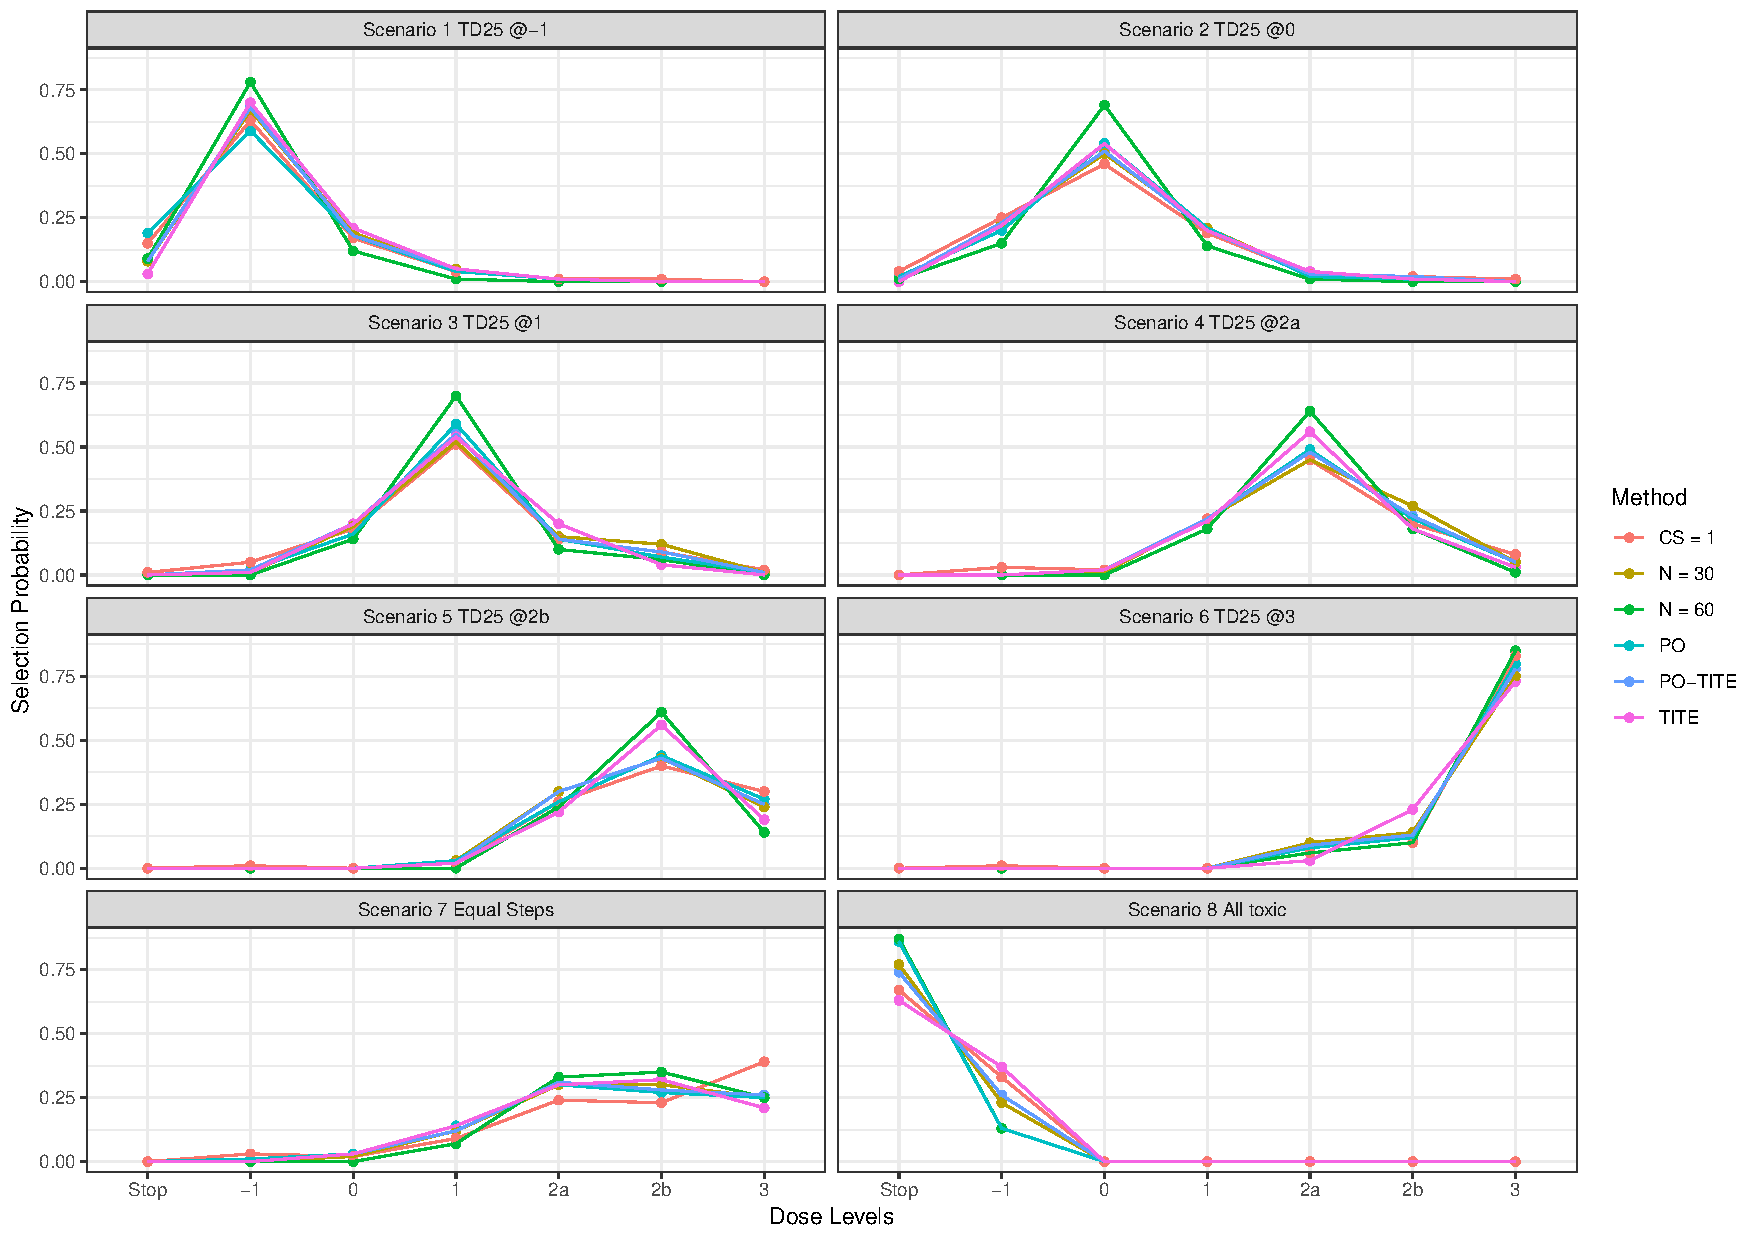
\includegraphics[width=\textwidth]{Adept-SimsOrder1}
\end{figure}

\begin{figure}[h!]
	\centering
	\caption[Plot of simulations comparing designs for ordering 2.]{Plot of the simulation results presented in Table \ref{tab_adept:Design_Comparison2} detailing selection probabilities for multiple designs across scenarios 9-16 (where 2a is considered more toxic than 2b).}
	\label{fig_adept:sims_order2}
	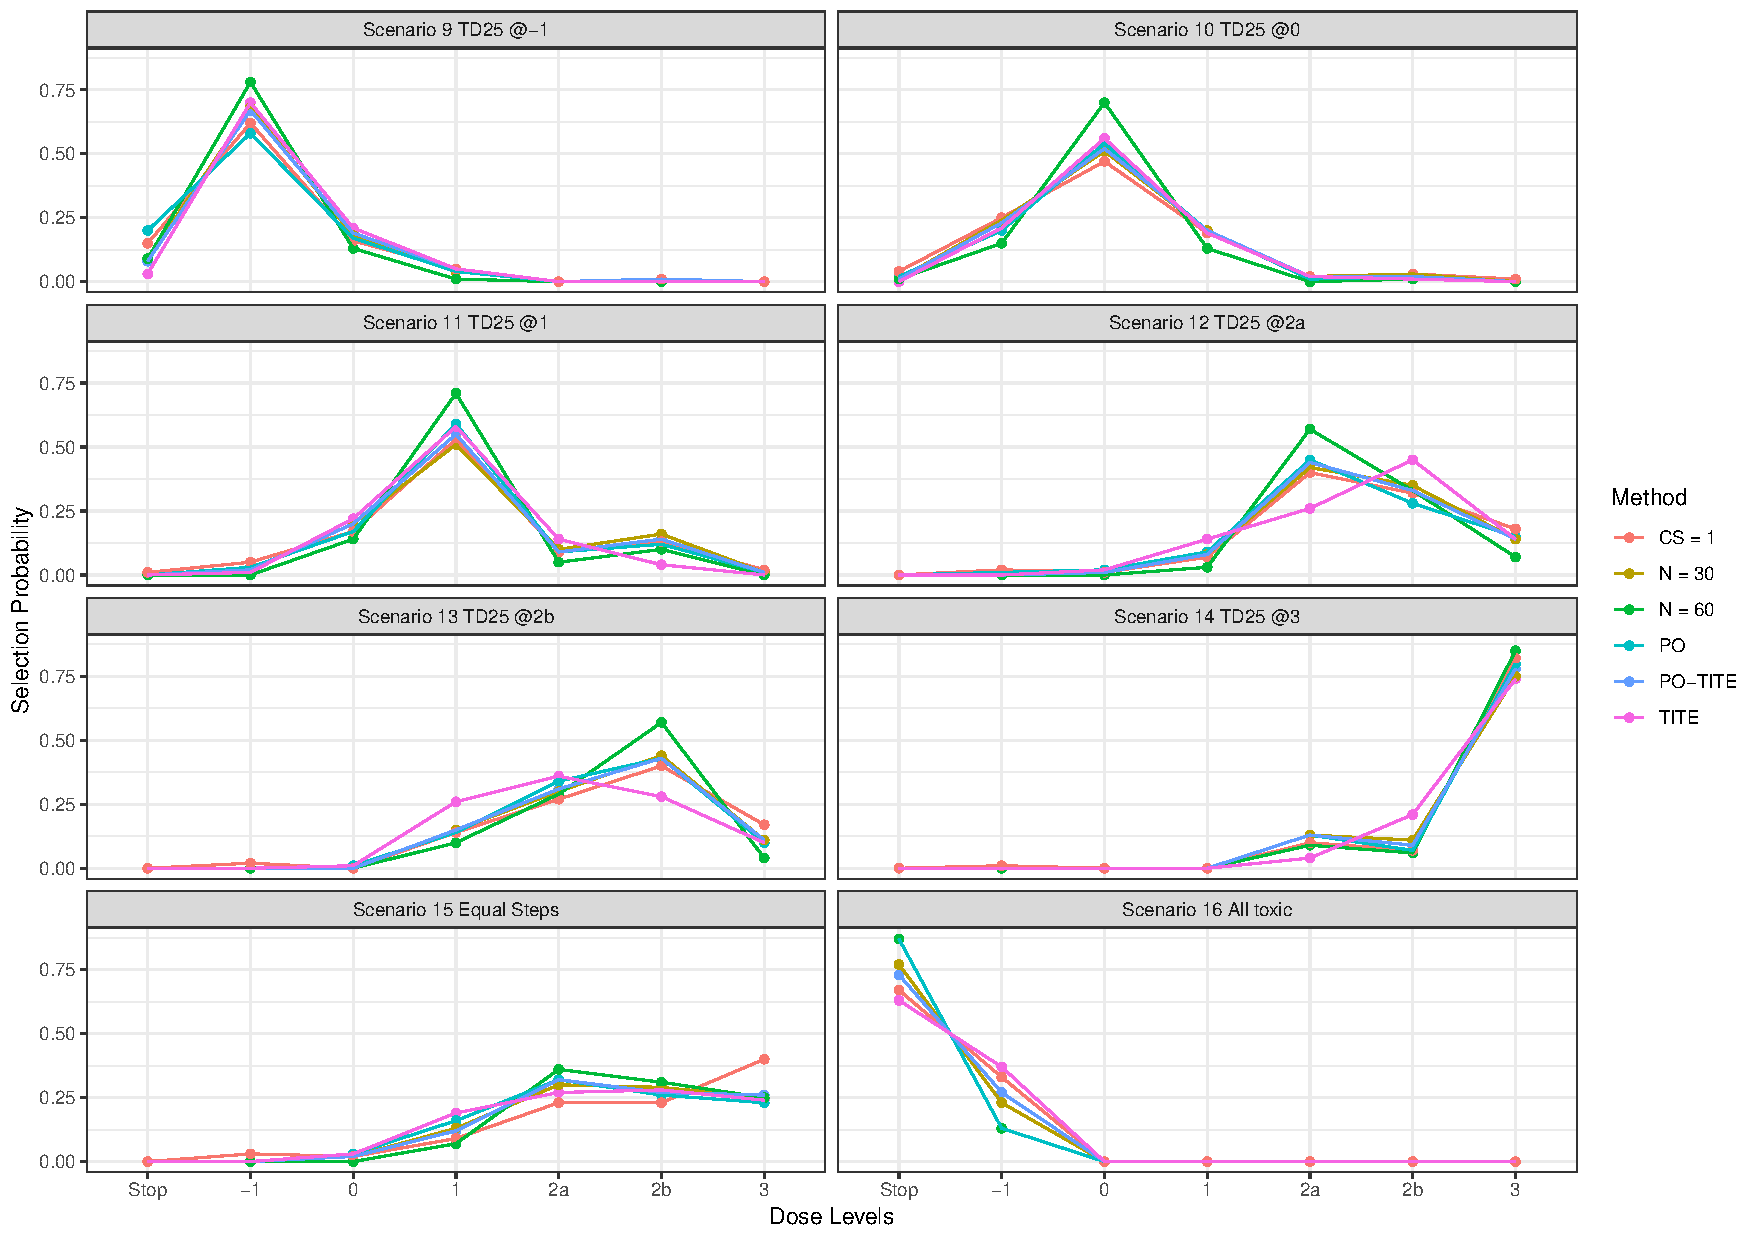
\includegraphics[width=\textwidth]{Adept-SimsOrder2}
\end{figure}

The TITE-CRM performs comparably to our original design for certain scenarios, specifically where 2a is assumed less toxic than 2b (Table \ref{tab_adept:OCorder1}). Compared to the PO-TITE design we see increases in probability selection for scenarios 4 and 5 where the target dose is at 2a and 2b respectively. This increase in performance can be attributed to the fact that the partial ordering no longer exists as we have assumed an ordering. The lower selection probabilities for the PO-TITE-CRM can be seen as the price to pay for the uncertainty of not knowing the order of 2a and 2b. However, the TITE-CRM underperforms in scenarios 9-16 where 2a is assumed more toxic than 2b. Specifically, scenarios 12 and 13 where it fails to identify the TD25 the majority of the time. This is also explored by Abbas et al. \cite{abbasComparisonPhaseDosefinding2020}. 

The PO-CRM design without a TITE component also performs similarly except for scenarios 1, 8, 9 and 16 where the trial stops more regularly for excess toxicity at the lowest dose. This would be because patients complete the full follow-up window before the next dose allocation decision is made. In a TITE setting a new cohort could be recruited before patients in previous cohorts experience a DLT. The main difference between these designs is the trial duration. Without the TITE component the trial duration is significantly longer, with the average length ranging from 70 to 195 months compared to 39 to 71 months for PO-TITE-CRM. In scenario 1 TITE-CRM duration is longer than the PO-TITE-CRM design this can be attributed to the lower chance of stopping early. If the trial is stopping early less it has more chance of going on for longer thus increasing the duration. 

The design with a fixed sample size of 30 is comparable to our design with the sample size of 60 and the consensus stopping rule. With a sample size of 30 selection probabilities are only 2-5\% lower. For the design with 60 patients, we see much improved operating characteristics with selection probabilities ranging from 31\% to 85\% for the various scenarios. Even though our original design specifies a sample size of 60 we rarely ever reach it as we often stop for consensus hence why this design performs better. The trade-off here is trial duration. Recruitment and follow-up under the constraints of these simulations will take much longer compared to our specification which is not ideal for an early-phase trial. Originally our design had a fixed sample size of 30 but as the clinicians wanted a dose expansion cohort we opted to use the consensus rule to ensure a minimum number of patients would be treated at the TD25. 

For the design with cohort size of one, we see somewhat comparable performance to that of the PO-TITE-CRM design. The design performs similarly for scenarios where the TD25 is at the lowest or highest dose level but underperforms for the more complex scenarios in terms of selection probabilities. This discrepancy in performance may be related to how the simulations recruit patients into the trial and the large DLT follow-up period, meaning more frequent dose allocation decisions are being made each with less available information. This also leads to the no cohorts design having a longer duration. Patients entered into the trial in cohorts of three will not have to wait the full minimum follow-up period between patients within the cohort.



%----------------------------------------------------------------------------------------
%	SECTION 5
%-------------------------.

\section{Discussion}  
\label{adept:Discussion}

The PO-CRM and PO-TITE-CRM designs offer solutions to the issue of partial ordering where the order of the treatments is only partially known. The original methodology details that this issue commonly arises in trials of multiple agents, where each drug individually may follow the monotonicity assumption but when combined at certain dose levels this may not hold. This issue is typically dealt with either by fixing the dose of one of the agents and escalating the other or escalating both agents simultaneously. This means certain drug combinations that are clinically relevant may not be investigated or even considered.  
 
Here we have shown that these issues can also arise in other situations. Even though the ADePT-DDR trial uses multiple agents, the issue of partial ordering occurs in this case due to the varying treatment dose and schedule for one of its agents AZD6738. Implementing the PO-TITE-CRM design allowed us to deal with this issue effectively. There may be other factors or variables in single-agent dose-finding trials that would lead to the issue of partial ordering and would warrant the use of either PO-CRM or PO-TITE-CRM. The issue of dose scheduling and partial ordering is further explored by Wages et al. \cite{wagesPhaseDesignCompletely2014} where they propose further methods for dealing with this issue. 

The limited literature review that was conducted highlighted that this may be the first instance of the PO-TITE-CRM design being applied. It is important to note that although this methodology takes into account all the various orderings, the main aim is to identify the TD and does not attempt to identify the order that is more correct. 

Compared to other CRM-based designs only a few additional pieces of information are required to implement the PO-CRM design. More important is the number of toxicity orderings and prior probabilities for the orders. Dependent on how many dose combinations are available it may not be feasible to investigate all combinations and all orderings. Careful thought and consideration should be given to the combinations and orderings selected which would require input from all relevant investigators. In terms of priors for orderings if no prior information is available, all orders should be treated as equally likely to occur. Extending this design to the PO-TITE-CRM requires a fit-for-purpose weight function and is applied similarly to the TITE-CRM methodology. There is an R package available with functions that can be used to run and simulate a PO-CRM trial. These functions were extended to included weighted dose-toxicity models as described in this chapter to implement PO-TITE-CRM into ADePT-DDR. The lack of available software for PO-TITE-CRM specifically may be one of the reasons for its lack of use.

In terms of ADePT-DDR, dose combinations were decided upon by the clinical investigators. The issue of partial ordering was due to the dose-levels 2a and 2b, as such this methodology was employed to deal with that scenario. This is a very simple example of partial ordering as we only have two possible orderings and six dose levels. The necessity of implementing this methodology was discussed and whether or not adopting an easier solution by simply altering the dose levels would have been better. Ultimately, the dose levels selected by the clinicians were deemed the most relevant with the TD25 likely to be one of these doses.     
 
Simulations and operating characteristics were the main tools used to assess the design's performance as well as help understand the impact of sample size and stopping rules. This was an iterative process that involved running multiple iterations of simulations under various scenarios until the design was finalised. A key point is that scenarios from simulations should account for each of the possible orderings. ADePT-DDR only has two orderings, we ran scenarios for both. For a trial with a greater number of orderings, this may be unfeasible but at least some scenarios should be assessed to ensure the design is behaving as expected. Overall, the design operating characteristics performed reasonably well even in difficult scenarios. 

One limitation of the simulations is how the time-to-event data is generated. The time of DLTs is sampled from a uniform distribution $U(0, 413)$, where the time of the DLT can occur at any time between the patient beginning treatment and the end of follow-up (413 days). Using this uniform distribution implies that a DLT has an equal probability of occurring at any time-point in the observation window. This may not be an accurate representation of what happens in the actual trial. Similar comments can be made about the accrual rate used in the simulations. Here we specified the recruitment of one patient per month which is in no way guaranteed for the actual trial. Wages et al. \cite{wagesUsingTimetoeventContinual2013}, when presenting this methodology investigated four different applications of the PO-TITE-CRM which used different models to enroll patients and allocate DLTs. Results across these four applications were comparable. 

The simulations are also able to instantaneously determine dose-levels for incoming cohorts with all available information. This does not fully reflect the process in which dose-escalation decisions would be made during the actual running of the trial. The analysis would require a data snapshot and time would have to be spent cleaning the data and determining the next dose-level. This would mean any data from the point of the snapshot would not be included in any dose escalation/de-escalation decisions. 

Similarly, there may also be limitations with some of the design choices made concerning cohort size and sample size. These were investigated alongside a variety of other trial designs that could have been implemented. This was done to validate the choices we made with the design and highlight the differences in operating characteristics due to the varying assumptions and components in the designs. The standard PO-CRM had a much longer average duration due to the lack of TITE component whereas a standard TITE-CRM overall performs better but assumes the ordering of toxicity is known. 

Here we have detailed the issue of partial ordering with a time-to-event component. We discuss how we implemented the trial design, in what we believe is the first real-world application of this specific design. A large amount of simulation work is required to assess the performance of the design. This is often an iterative process to refine decisions that were made and often requires input from both clinical and statistical investigators. We recommend running several varied scenarios for each potential ordering that will be investigated. Finally, we also compared the implementation of PO-TITE-CRM to various other designs and showed it performs relatively well given all of the methodological and practical challenges. 

